\documentclass[twoside]{book}

% Packages required by doxygen
\usepackage{calc}
\usepackage{doxygen}
\usepackage{graphicx}
\usepackage[utf8]{inputenc}
\usepackage{makeidx}
\usepackage{multicol}
\usepackage{multirow}
\usepackage{textcomp}
\usepackage[table]{xcolor}

% Font selection
\usepackage[T1]{fontenc}
\usepackage{mathptmx}
\usepackage[scaled=.90]{helvet}
\usepackage{courier}
\usepackage{amssymb}
\usepackage{sectsty}
\renewcommand{\familydefault}{\sfdefault}
\allsectionsfont{%
  \fontseries{bc}\selectfont%
  \color{darkgray}%
}
\renewcommand{\DoxyLabelFont}{%
  \fontseries{bc}\selectfont%
  \color{darkgray}%
}

% Page & text layout
\usepackage{geometry}
\geometry{%
  a4paper,%
  top=2.5cm,%
  bottom=2.5cm,%
  left=2.5cm,%
  right=2.5cm%
}
\tolerance=750
\hfuzz=15pt
\hbadness=750
\setlength{\emergencystretch}{15pt}
\setlength{\parindent}{0cm}
\setlength{\parskip}{0.2cm}
\makeatletter
\renewcommand{\paragraph}{%
  \@startsection{paragraph}{4}{0ex}{-1.0ex}{1.0ex}{%
    \normalfont\normalsize\bfseries\SS@parafont%
  }%
}
\renewcommand{\subparagraph}{%
  \@startsection{subparagraph}{5}{0ex}{-1.0ex}{1.0ex}{%
    \normalfont\normalsize\bfseries\SS@subparafont%
  }%
}
\makeatother

% Headers & footers
\usepackage{fancyhdr}
\pagestyle{fancyplain}
\fancyhead[LE]{\fancyplain{}{\bfseries\thepage}}
\fancyhead[CE]{\fancyplain{}{}}
\fancyhead[RE]{\fancyplain{}{\bfseries\leftmark}}
\fancyhead[LO]{\fancyplain{}{\bfseries\rightmark}}
\fancyhead[CO]{\fancyplain{}{}}
\fancyhead[RO]{\fancyplain{}{\bfseries\thepage}}
\fancyfoot[LE]{\fancyplain{}{}}
\fancyfoot[CE]{\fancyplain{}{}}
\fancyfoot[RE]{\fancyplain{}{\bfseries\scriptsize Generated on Sun Apr 27 2014 12\-:59\-:38 for Alien\-Hunt by Doxygen }}
\fancyfoot[LO]{\fancyplain{}{\bfseries\scriptsize Generated on Sun Apr 27 2014 12\-:59\-:38 for Alien\-Hunt by Doxygen }}
\fancyfoot[CO]{\fancyplain{}{}}
\fancyfoot[RO]{\fancyplain{}{}}
\renewcommand{\footrulewidth}{0.4pt}
\renewcommand{\chaptermark}[1]{%
  \markboth{#1}{}%
}
\renewcommand{\sectionmark}[1]{%
  \markright{\thesection\ #1}%
}

% Indices & bibliography
\usepackage{natbib}
\usepackage[titles]{tocloft}
\setcounter{tocdepth}{3}
\setcounter{secnumdepth}{5}
\makeindex

% Hyperlinks (required, but should be loaded last)
\usepackage{ifpdf}
\ifpdf
  \usepackage[pdftex,pagebackref=true]{hyperref}
\else
  \usepackage[ps2pdf,pagebackref=true]{hyperref}
\fi
\hypersetup{%
  colorlinks=true,%
  linkcolor=blue,%
  citecolor=blue,%
  unicode%
}

% Custom commands
\newcommand{\clearemptydoublepage}{%
  \newpage{\pagestyle{empty}\cleardoublepage}%
}


%===== C O N T E N T S =====

\begin{document}

% Titlepage & ToC
\hypersetup{pageanchor=false}
\pagenumbering{roman}
\begin{titlepage}
\vspace*{7cm}
\begin{center}%
{\Large Alien\-Hunt }\\
\vspace*{1cm}
{\large Generated by Doxygen 1.8.6}\\
\vspace*{0.5cm}
{\small Sun Apr 27 2014 12:59:38}\\
\end{center}
\end{titlepage}
\clearemptydoublepage
\tableofcontents
\clearemptydoublepage
\pagenumbering{arabic}
\hypersetup{pageanchor=true}

%--- Begin generated contents ---
\chapter{Bug List}
\label{bug}
\hypertarget{bug}{}

\begin{DoxyRefList}
\item[\label{bug__bug000001}%
\hypertarget{bug__bug000001}{}%
Class \hyperlink{class_door_sensor_script}{Door\-Sensor\-Script} ]sound doesn't play completely when level is loaded  
\item[\label{bug__bug000002}%
\hypertarget{bug__bug000002}{}%
Class \hyperlink{class_l1_player_script}{L1\-Player\-Script} ]audio is cut off when level 2 is loaded  
\item[\label{bug__bug000003}%
\hypertarget{bug__bug000003}{}%
Class \hyperlink{class_l2_ship_sensor}{L2\-Ship\-Sensor} ]audio is skipped when game level is loaded  
\item[\label{bug__bug000004}%
\hypertarget{bug__bug000004}{}%
Class \hyperlink{class_player}{Player} ]if player loses all his lives the audio is interrupted by the new level loaded  
\item[\label{bug__bug000005}%
\hypertarget{bug__bug000005}{}%
Class \hyperlink{class_ship_sensor}{Ship\-Sensor} ]audio is skipped when game level is loaded 
\end{DoxyRefList}
\chapter{Hierarchical Index}
\section{Class Hierarchy}
This inheritance list is sorted roughly, but not completely, alphabetically\-:\begin{DoxyCompactList}
\item Mono\-Behaviour\begin{DoxyCompactList}
\item \contentsline{section}{Badguy\-Script}{\pageref{class_badguy_script}}{}
\item \contentsline{section}{Destroy\-When\-Hit}{\pageref{class_destroy_when_hit}}{}
\item \contentsline{section}{Door\-Sensor\-Script}{\pageref{class_door_sensor_script}}{}
\item \contentsline{section}{Fading\-Message}{\pageref{class_fading_message}}{}
\item \contentsline{section}{Game\-Won\-Behaviour}{\pageref{class_game_won_behaviour}}{}
\item \contentsline{section}{Game\-Won\-Rollover}{\pageref{class_game_won_rollover}}{}
\item \contentsline{section}{Instructions\-Rollover\-Menu}{\pageref{class_instructions_rollover_menu}}{}
\item \contentsline{section}{L1\-Player\-Script}{\pageref{class_l1_player_script}}{}
\item \contentsline{section}{L2\-Player}{\pageref{class_l2_player}}{}
\item \contentsline{section}{L2\-Player\-Engine\-Icon}{\pageref{class_l2_player_engine_icon}}{}
\item \contentsline{section}{L2\-Player\-G\-U\-I}{\pageref{class_l2_player_g_u_i}}{}
\item \contentsline{section}{L2\-Ship\-Sensor}{\pageref{class_l2_ship_sensor}}{}
\item \contentsline{section}{Player}{\pageref{class_player}}{}
\item \contentsline{section}{Player\-Engine\-Icon}{\pageref{class_player_engine_icon}}{}
\item \contentsline{section}{Player\-G\-U\-I}{\pageref{class_player_g_u_i}}{}
\item \contentsline{section}{Player\-Inventory\-Icon}{\pageref{class_player_inventory_icon}}{}
\item \contentsline{section}{Play\-Rollover\-Menu}{\pageref{class_play_rollover_menu}}{}
\item \contentsline{section}{Rollover\-Game\-Over}{\pageref{class_rollover_game_over}}{}
\item \contentsline{section}{Ship\-Sensor}{\pageref{class_ship_sensor}}{}
\item \contentsline{section}{Third\-Person\-Camera}{\pageref{class_third_person_camera}}{}
\end{DoxyCompactList}
\end{DoxyCompactList}

\chapter{Class Index}
\section{Class List}
Here are the classes, structs, unions and interfaces with brief descriptions\-:\begin{DoxyCompactList}
\item\contentsline{section}{\hyperlink{class_badguy_script}{Badguy\-Script} \\*Class to control the movement of the Badguy prefab }{\pageref{class_badguy_script}}{}
\item\contentsline{section}{\hyperlink{class_destroy_when_hit}{Destroy\-When\-Hit} \\*Destroys the game object when the trigger is entered }{\pageref{class_destroy_when_hit}}{}
\item\contentsline{section}{\hyperlink{class_door_sensor_script}{Door\-Sensor\-Script} \\*Controls the interaction of player and the door }{\pageref{class_door_sensor_script}}{}
\item\contentsline{section}{\hyperlink{class_fading_message}{Fading\-Message} \\*Prefab object that displays a message that fades on screen }{\pageref{class_fading_message}}{}
\item\contentsline{section}{\hyperlink{class_game_won_behaviour}{Game\-Won\-Behaviour} }{\pageref{class_game_won_behaviour}}{}
\item\contentsline{section}{\hyperlink{class_game_won_rollover}{Game\-Won\-Rollover} \\*Interacts with the actions of the user after completing the game }{\pageref{class_game_won_rollover}}{}
\item\contentsline{section}{\hyperlink{class_instructions_rollover_menu}{Instructions\-Rollover\-Menu} \\*Interacts with the actions of the user to enter the instructions scene }{\pageref{class_instructions_rollover_menu}}{}
\item\contentsline{section}{\hyperlink{class_l1_player_script}{L1\-Player\-Script} \\*Class that controls the \hyperlink{class_player}{Player} on level 1 }{\pageref{class_l1_player_script}}{}
\item\contentsline{section}{\hyperlink{class_l2_player}{L2\-Player} \\*Class that controls the \hyperlink{class_player}{Player} on level 2 }{\pageref{class_l2_player}}{}
\item\contentsline{section}{\hyperlink{class_l2_player_engine_icon}{L2\-Player\-Engine\-Icon} \\*Class that displays the engine icons on the screen }{\pageref{class_l2_player_engine_icon}}{}
\item\contentsline{section}{\hyperlink{class_l2_player_g_u_i}{L2\-Player\-G\-U\-I} \\*Class that displays the players lives left on level 2 }{\pageref{class_l2_player_g_u_i}}{}
\item\contentsline{section}{\hyperlink{class_l2_ship_sensor}{L2\-Ship\-Sensor} \\*Controls whether the player collected all the parts needed to fix the ship when trigger is entered }{\pageref{class_l2_ship_sensor}}{}
\item\contentsline{section}{\hyperlink{class_player}{Player} \\*Class that controls the player for level 3 }{\pageref{class_player}}{}
\item\contentsline{section}{\hyperlink{class_player_engine_icon}{Player\-Engine\-Icon} \\*Class that displays the engine icons on the screen }{\pageref{class_player_engine_icon}}{}
\item\contentsline{section}{\hyperlink{class_player_g_u_i}{Player\-G\-U\-I} \\*Class that displays the players lives left on level 3 }{\pageref{class_player_g_u_i}}{}
\item\contentsline{section}{\hyperlink{class_player_inventory_icon}{Player\-Inventory\-Icon} \\*Class that manages the display of the key icon if the player has the key or not }{\pageref{class_player_inventory_icon}}{}
\item\contentsline{section}{\hyperlink{class_play_rollover_menu}{Play\-Rollover\-Menu} \\*Interacts with the actions of the user when starting the game }{\pageref{class_play_rollover_menu}}{}
\item\contentsline{section}{\hyperlink{class_rollover_game_over}{Rollover\-Game\-Over} \\*Interacts with the actions of the user after losing all your lives }{\pageref{class_rollover_game_over}}{}
\item\contentsline{section}{\hyperlink{class_ship_sensor}{Ship\-Sensor} \\*Controls whether the player collected all the parts needed to fix the ship when trigger is entered }{\pageref{class_ship_sensor}}{}
\item\contentsline{section}{\hyperlink{class_third_person_camera}{Third\-Person\-Camera} }{\pageref{class_third_person_camera}}{}
\end{DoxyCompactList}

\chapter{Class Documentation}
\hypertarget{class_badguy_script}{\section{Badguy\-Script Class Reference}
\label{class_badguy_script}\index{Badguy\-Script@{Badguy\-Script}}
}


Class to control the movement of the Badguy prefab.  


Inheritance diagram for Badguy\-Script\-:\begin{figure}[H]
\begin{center}
\leavevmode
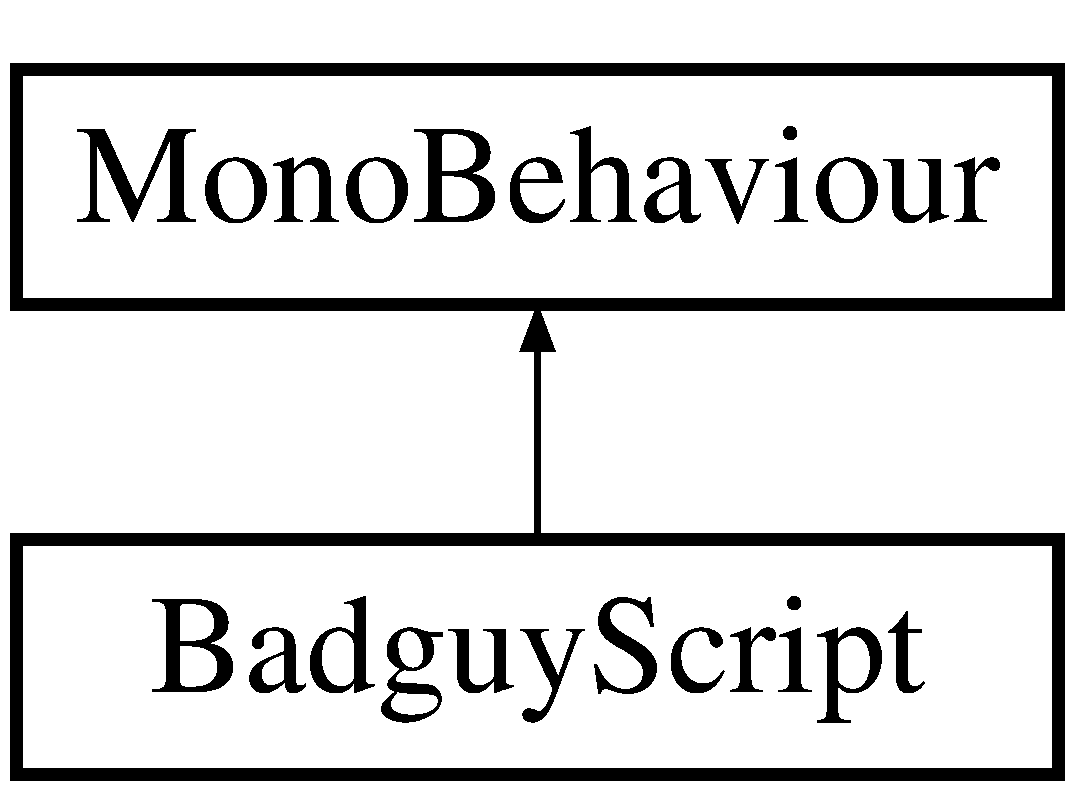
\includegraphics[height=2.000000cm]{class_badguy_script}
\end{center}
\end{figure}
\subsection*{Public Attributes}
\begin{DoxyCompactItemize}
\item 
float \hyperlink{class_badguy_script_a54a3b82f3f8a72ac65c2ef9de4d4bb67}{x\-Movement\-Per\-Second} = 1f
\item 
float \hyperlink{class_badguy_script_a4c4bd91ecd881d121488e41bafea8d14}{min\-X} = 0f
\item 
float \hyperlink{class_badguy_script_a25c3c2d6c4f4458d7dceb9eb6e69d7c0}{max\-X} = 10f
\end{DoxyCompactItemize}


\subsection{Detailed Description}
Class to control the movement of the Badguy prefab. 

\begin{DoxyAuthor}{Author}
David Kelly 
\end{DoxyAuthor}
\begin{DoxyVersion}{Version}
1.\-0 
\end{DoxyVersion}
\begin{DoxyDate}{Date}
20/4/14 
\end{DoxyDate}


\subsection{Member Data Documentation}
\hypertarget{class_badguy_script_a25c3c2d6c4f4458d7dceb9eb6e69d7c0}{\index{Badguy\-Script@{Badguy\-Script}!max\-X@{max\-X}}
\index{max\-X@{max\-X}!BadguyScript@{Badguy\-Script}}
\subsubsection[{max\-X}]{\setlength{\rightskip}{0pt plus 5cm}float Badguy\-Script.\-max\-X = 10f}}\label{class_badguy_script_a25c3c2d6c4f4458d7dceb9eb6e69d7c0}
A public variable to control the maximum value on the X axis the Badguy prefab can move between \hypertarget{class_badguy_script_a4c4bd91ecd881d121488e41bafea8d14}{\index{Badguy\-Script@{Badguy\-Script}!min\-X@{min\-X}}
\index{min\-X@{min\-X}!BadguyScript@{Badguy\-Script}}
\subsubsection[{min\-X}]{\setlength{\rightskip}{0pt plus 5cm}float Badguy\-Script.\-min\-X = 0f}}\label{class_badguy_script_a4c4bd91ecd881d121488e41bafea8d14}
A public variable to control the minimum value on the X axis the Badguy prefab can move between \hypertarget{class_badguy_script_a54a3b82f3f8a72ac65c2ef9de4d4bb67}{\index{Badguy\-Script@{Badguy\-Script}!x\-Movement\-Per\-Second@{x\-Movement\-Per\-Second}}
\index{x\-Movement\-Per\-Second@{x\-Movement\-Per\-Second}!BadguyScript@{Badguy\-Script}}
\subsubsection[{x\-Movement\-Per\-Second}]{\setlength{\rightskip}{0pt plus 5cm}float Badguy\-Script.\-x\-Movement\-Per\-Second = 1f}}\label{class_badguy_script_a54a3b82f3f8a72ac65c2ef9de4d4bb67}
A public variable to control the speed the Badguy prefab moves 

The documentation for this class was generated from the following file\-:\begin{DoxyCompactItemize}
\item 
Badguy\-Script.\-cs\end{DoxyCompactItemize}

\hypertarget{class_destroy_when_hit}{\section{Destroy\-When\-Hit Class Reference}
\label{class_destroy_when_hit}\index{Destroy\-When\-Hit@{Destroy\-When\-Hit}}
}


Destroys the game object when the trigger is entered.  


Inheritance diagram for Destroy\-When\-Hit\-:\begin{figure}[H]
\begin{center}
\leavevmode
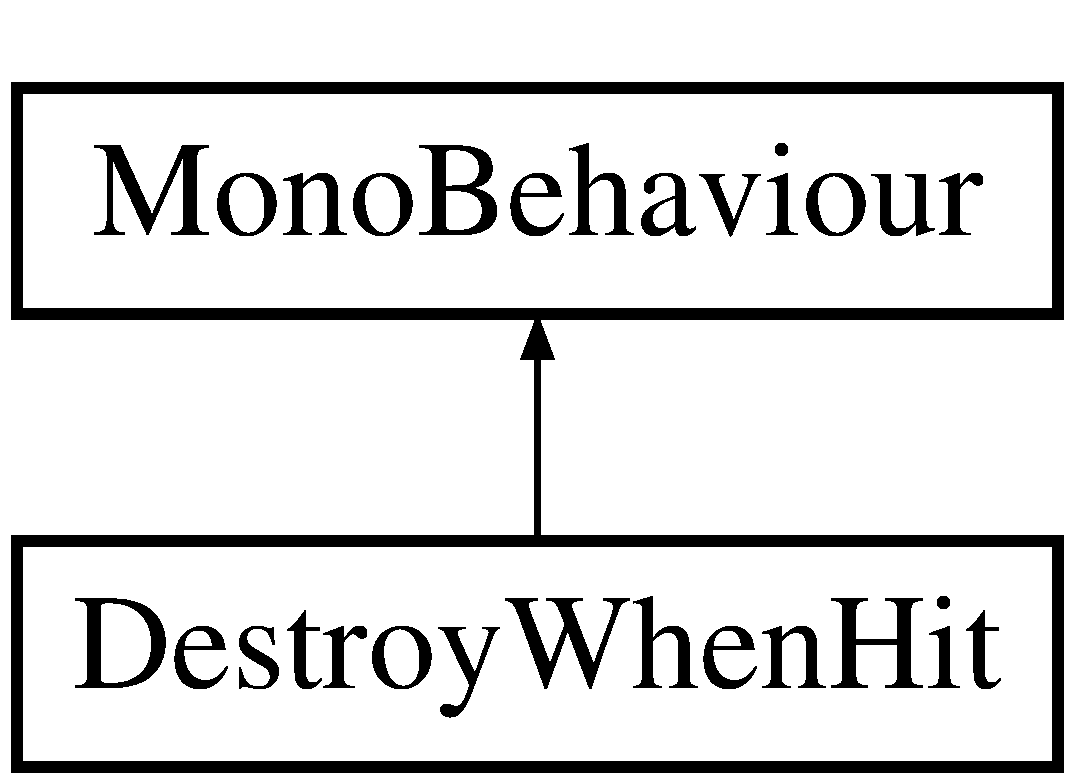
\includegraphics[height=2.000000cm]{class_destroy_when_hit}
\end{center}
\end{figure}


\subsection{Detailed Description}
Destroys the game object when the trigger is entered. 

\begin{DoxyAuthor}{Author}
David Kelly 
\end{DoxyAuthor}
\begin{DoxyVersion}{Version}
1.\-0 
\end{DoxyVersion}
\begin{DoxyDate}{Date}
20/4/14 
\end{DoxyDate}


The documentation for this class was generated from the following file\-:\begin{DoxyCompactItemize}
\item 
Destroy\-When\-Hit.\-cs\end{DoxyCompactItemize}

\hypertarget{class_door_sensor_script}{\section{Door\-Sensor\-Script Class Reference}
\label{class_door_sensor_script}\index{Door\-Sensor\-Script@{Door\-Sensor\-Script}}
}


Controls the interaction of player and the door.  


Inheritance diagram for Door\-Sensor\-Script\-:\begin{figure}[H]
\begin{center}
\leavevmode
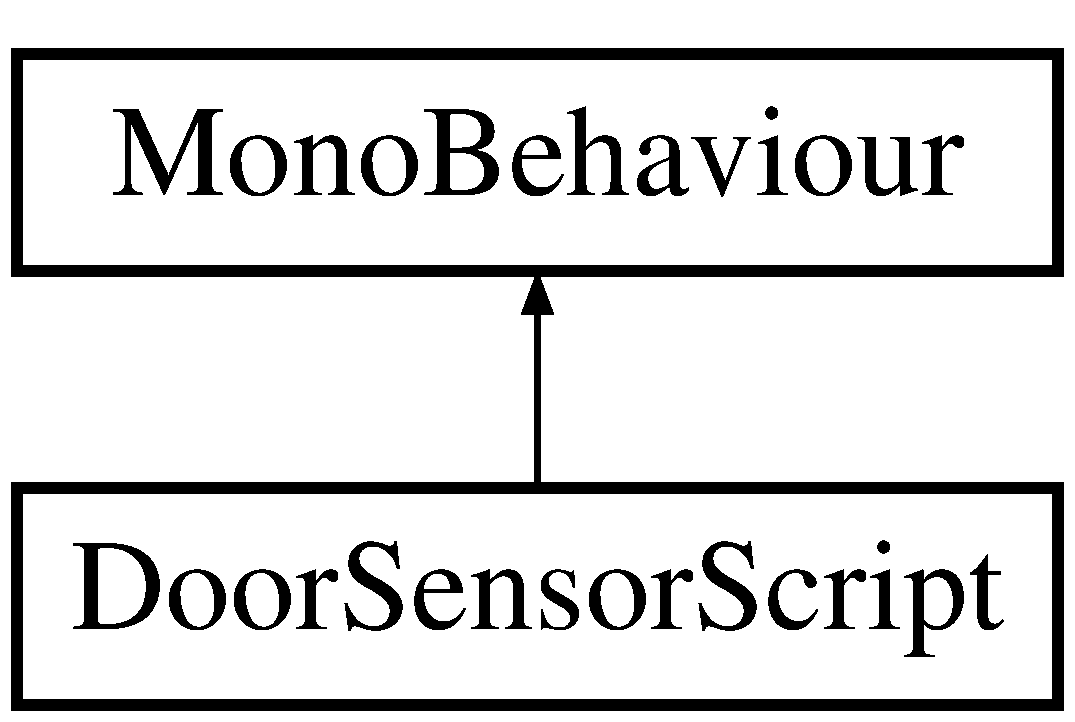
\includegraphics[height=2.000000cm]{class_door_sensor_script}
\end{center}
\end{figure}
\subsection*{Public Attributes}
\begin{DoxyCompactItemize}
\item 
Game\-Object \hyperlink{class_door_sensor_script_a3ac7f794c8f0553a80a7ff9f5ea1717a}{cube\-G\-O}
\item 
Audio\-Clip \hyperlink{class_door_sensor_script_a8cdc54e500df0194633b1aa6830460a9}{Close}
\item 
Audio\-Clip \hyperlink{class_door_sensor_script_a5e5b72d9a89f93da35dcd2377f0435c0}{Open}
\item 
Game\-Object \hyperlink{class_door_sensor_script_abeeac4e7d1793824f6eacb8939e746be}{fading\-Message\-Prefab}
\item 
\hypertarget{class_door_sensor_script_a481e3e75882a1f9e4c382bd134d0ba14}{string {\bfseries message\-Text} = \char`\"{}(message to appear)\char`\"{}}\label{class_door_sensor_script_a481e3e75882a1f9e4c382bd134d0ba14}

\end{DoxyCompactItemize}


\subsection{Detailed Description}
Controls the interaction of player and the door. 

\begin{DoxyAuthor}{Author}
David Kelly 
\end{DoxyAuthor}
\begin{DoxyVersion}{Version}
1.\-0 
\end{DoxyVersion}
\begin{DoxyDate}{Date}
20/4/14
\end{DoxyDate}
\begin{DoxyWarning}{Warning}
player must have collected the items being returned from the player class
\end{DoxyWarning}
\begin{DoxyRefDesc}{Bug}
\item[\hyperlink{bug__bug000001}{Bug}]sound doesn't play completely when level is loaded \end{DoxyRefDesc}


\subsection{Member Data Documentation}
\hypertarget{class_door_sensor_script_a8cdc54e500df0194633b1aa6830460a9}{\index{Door\-Sensor\-Script@{Door\-Sensor\-Script}!Close@{Close}}
\index{Close@{Close}!DoorSensorScript@{Door\-Sensor\-Script}}
\subsubsection[{Close}]{\setlength{\rightskip}{0pt plus 5cm}Audio\-Clip Door\-Sensor\-Script.\-Close}}\label{class_door_sensor_script_a8cdc54e500df0194633b1aa6830460a9}
Creating an audio file to reference \hypertarget{class_door_sensor_script_a3ac7f794c8f0553a80a7ff9f5ea1717a}{\index{Door\-Sensor\-Script@{Door\-Sensor\-Script}!cube\-G\-O@{cube\-G\-O}}
\index{cube\-G\-O@{cube\-G\-O}!DoorSensorScript@{Door\-Sensor\-Script}}
\subsubsection[{cube\-G\-O}]{\setlength{\rightskip}{0pt plus 5cm}Game\-Object Door\-Sensor\-Script.\-cube\-G\-O}}\label{class_door_sensor_script_a3ac7f794c8f0553a80a7ff9f5ea1717a}
Creating a game object to reference \hypertarget{class_door_sensor_script_abeeac4e7d1793824f6eacb8939e746be}{\index{Door\-Sensor\-Script@{Door\-Sensor\-Script}!fading\-Message\-Prefab@{fading\-Message\-Prefab}}
\index{fading\-Message\-Prefab@{fading\-Message\-Prefab}!DoorSensorScript@{Door\-Sensor\-Script}}
\subsubsection[{fading\-Message\-Prefab}]{\setlength{\rightskip}{0pt plus 5cm}Game\-Object Door\-Sensor\-Script.\-fading\-Message\-Prefab}}\label{class_door_sensor_script_abeeac4e7d1793824f6eacb8939e746be}
Creating a message prefab reference \hypertarget{class_door_sensor_script_a5e5b72d9a89f93da35dcd2377f0435c0}{\index{Door\-Sensor\-Script@{Door\-Sensor\-Script}!Open@{Open}}
\index{Open@{Open}!DoorSensorScript@{Door\-Sensor\-Script}}
\subsubsection[{Open}]{\setlength{\rightskip}{0pt plus 5cm}Audio\-Clip Door\-Sensor\-Script.\-Open}}\label{class_door_sensor_script_a5e5b72d9a89f93da35dcd2377f0435c0}
Creating an audio file to reference 

The documentation for this class was generated from the following file\-:\begin{DoxyCompactItemize}
\item 
Door\-Sensor\-Script.\-cs\end{DoxyCompactItemize}

\hypertarget{class_fading_message}{\section{Fading\-Message Class Reference}
\label{class_fading_message}\index{Fading\-Message@{Fading\-Message}}
}


Prefab object that displays a message that fades on screen.  


Inheritance diagram for Fading\-Message\-:\begin{figure}[H]
\begin{center}
\leavevmode
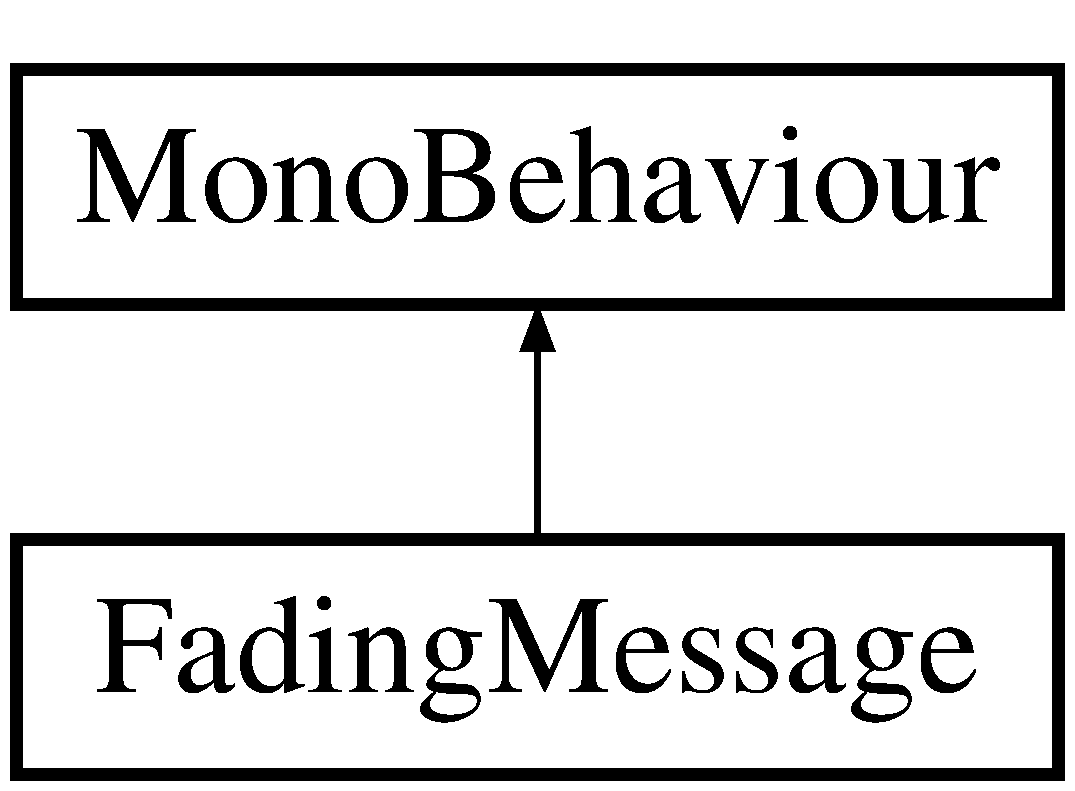
\includegraphics[height=2.000000cm]{class_fading_message}
\end{center}
\end{figure}


\subsection{Detailed Description}
Prefab object that displays a message that fades on screen. 

\begin{DoxyAuthor}{Author}
David Kelly 
\end{DoxyAuthor}
\begin{DoxyVersion}{Version}
1.\-0 
\end{DoxyVersion}
\begin{DoxyDate}{Date}
20/4/14 
\end{DoxyDate}


The documentation for this class was generated from the following file\-:\begin{DoxyCompactItemize}
\item 
Fading\-Message.\-cs\end{DoxyCompactItemize}

\hypertarget{class_game_won_behaviour}{\section{Game\-Won\-Behaviour Class Reference}
\label{class_game_won_behaviour}\index{Game\-Won\-Behaviour@{Game\-Won\-Behaviour}}
}
Inheritance diagram for Game\-Won\-Behaviour\-:\begin{figure}[H]
\begin{center}
\leavevmode
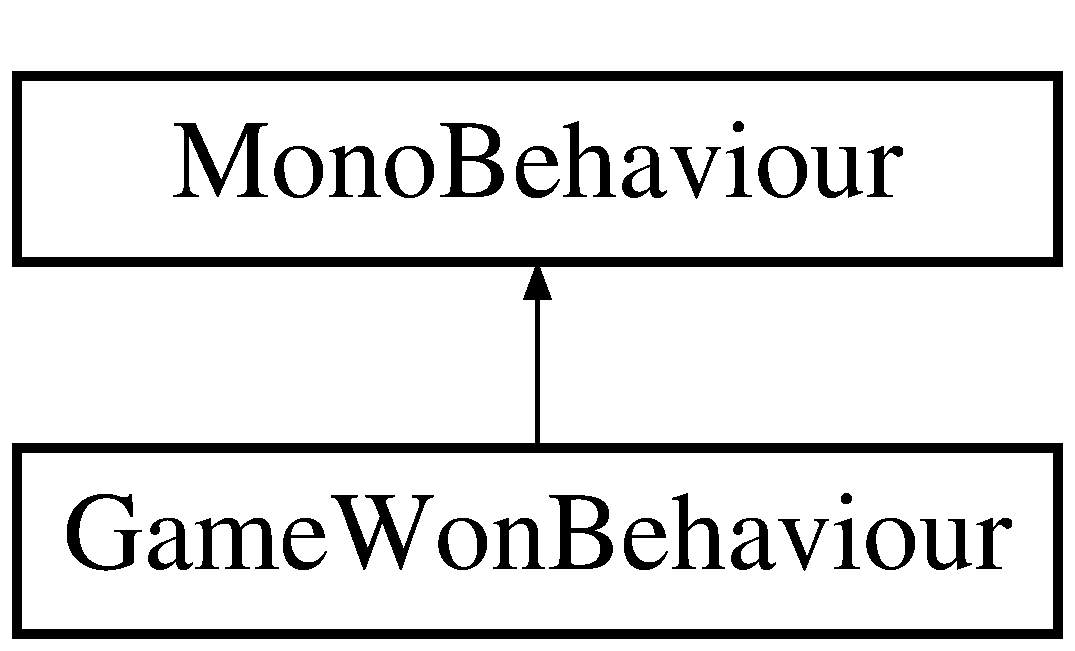
\includegraphics[height=2.000000cm]{class_game_won_behaviour}
\end{center}
\end{figure}
\subsection*{Public Member Functions}
\begin{DoxyCompactItemize}
\item 
\hypertarget{class_game_won_behaviour_a238fa3e09a1eae4d031cccac39fc7cdf}{void {\bfseries Play\-Sound} ()}\label{class_game_won_behaviour_a238fa3e09a1eae4d031cccac39fc7cdf}

\end{DoxyCompactItemize}


The documentation for this class was generated from the following file\-:\begin{DoxyCompactItemize}
\item 
Game\-Won\-Behaviour.\-cs\end{DoxyCompactItemize}

\hypertarget{class_game_won_rollover}{\section{Game\-Won\-Rollover Class Reference}
\label{class_game_won_rollover}\index{Game\-Won\-Rollover@{Game\-Won\-Rollover}}
}


Interacts with the actions of the user after completing the game.  


Inheritance diagram for Game\-Won\-Rollover\-:\begin{figure}[H]
\begin{center}
\leavevmode
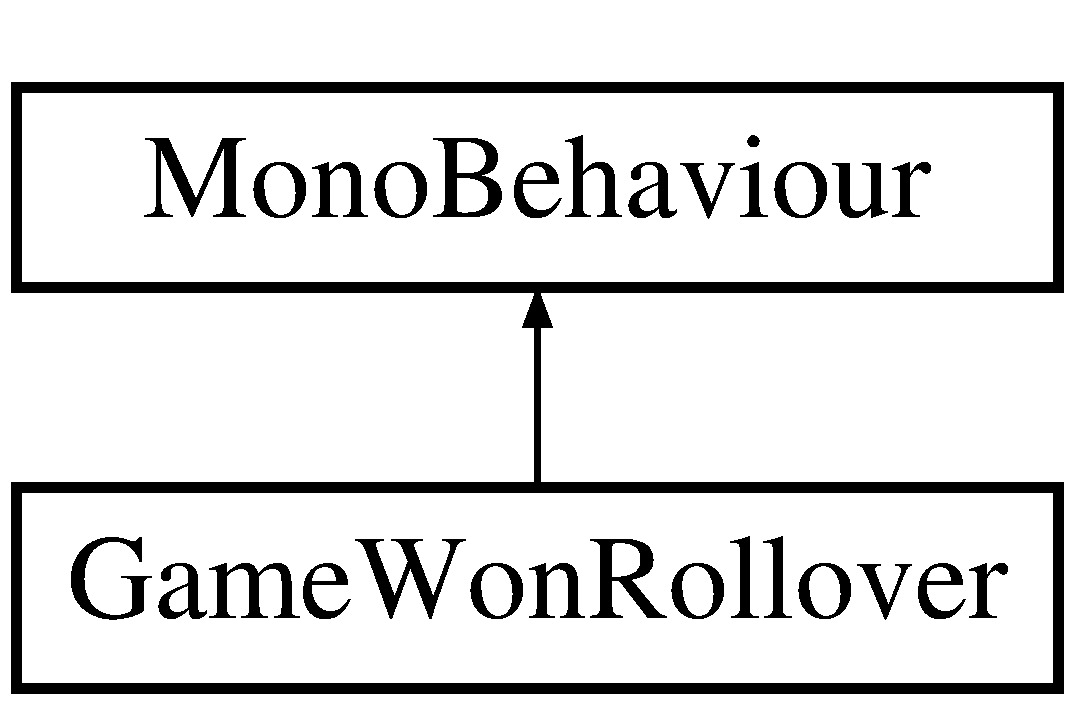
\includegraphics[height=2.000000cm]{class_game_won_rollover}
\end{center}
\end{figure}
\subsection*{Public Attributes}
\begin{DoxyCompactItemize}
\item 
Texture2\-D \hyperlink{class_game_won_rollover_a34f70647ed3d11b473719789f3a70d17}{normal\-Image}
\item 
Texture2\-D \hyperlink{class_game_won_rollover_a8fdd8cbd840e471566a0731f80e96a57}{rollover\-Image}
\end{DoxyCompactItemize}


\subsection{Detailed Description}
Interacts with the actions of the user after completing the game. 

\begin{DoxyAuthor}{Author}
David Kelly 
\end{DoxyAuthor}
\begin{DoxyVersion}{Version}
1.\-0 
\end{DoxyVersion}
\begin{DoxyDate}{Date}
20/4/14 
\end{DoxyDate}


\subsection{Member Data Documentation}
\hypertarget{class_game_won_rollover_a34f70647ed3d11b473719789f3a70d17}{\index{Game\-Won\-Rollover@{Game\-Won\-Rollover}!normal\-Image@{normal\-Image}}
\index{normal\-Image@{normal\-Image}!GameWonRollover@{Game\-Won\-Rollover}}
\subsubsection[{normal\-Image}]{\setlength{\rightskip}{0pt plus 5cm}Texture2\-D Game\-Won\-Rollover.\-normal\-Image}}\label{class_game_won_rollover_a34f70647ed3d11b473719789f3a70d17}
Reference to image to be displayed \hypertarget{class_game_won_rollover_a8fdd8cbd840e471566a0731f80e96a57}{\index{Game\-Won\-Rollover@{Game\-Won\-Rollover}!rollover\-Image@{rollover\-Image}}
\index{rollover\-Image@{rollover\-Image}!GameWonRollover@{Game\-Won\-Rollover}}
\subsubsection[{rollover\-Image}]{\setlength{\rightskip}{0pt plus 5cm}Texture2\-D Game\-Won\-Rollover.\-rollover\-Image}}\label{class_game_won_rollover_a8fdd8cbd840e471566a0731f80e96a57}
Reference to image to be displayed 

The documentation for this class was generated from the following file\-:\begin{DoxyCompactItemize}
\item 
Game\-Won\-Rollover.\-cs\end{DoxyCompactItemize}

\hypertarget{class_instructions_rollover_menu}{\section{Instructions\-Rollover\-Menu Class Reference}
\label{class_instructions_rollover_menu}\index{Instructions\-Rollover\-Menu@{Instructions\-Rollover\-Menu}}
}


Interacts with the actions of the user to enter the instructions scene.  


Inheritance diagram for Instructions\-Rollover\-Menu\-:\begin{figure}[H]
\begin{center}
\leavevmode
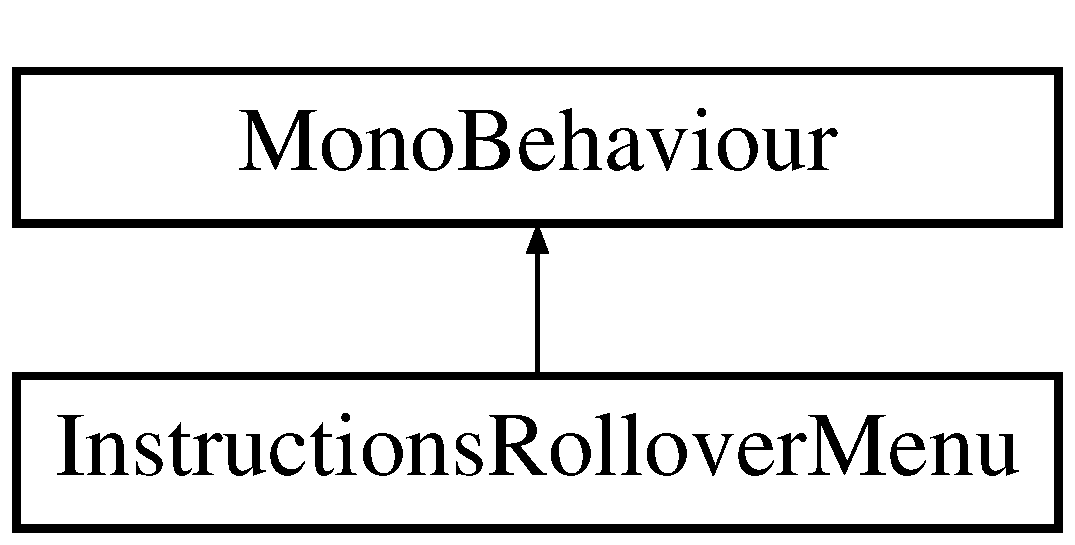
\includegraphics[height=2.000000cm]{class_instructions_rollover_menu}
\end{center}
\end{figure}
\subsection*{Public Attributes}
\begin{DoxyCompactItemize}
\item 
Texture2\-D \hyperlink{class_instructions_rollover_menu_abc4315ea253fbea4491da43647f1aae2}{normal\-Image}
\item 
Texture2\-D \hyperlink{class_instructions_rollover_menu_a858d6b4b9e15fcb415a51561845618ef}{rollover\-Image}
\end{DoxyCompactItemize}


\subsection{Detailed Description}
Interacts with the actions of the user to enter the instructions scene. 

\begin{DoxyAuthor}{Author}
David Kelly 
\end{DoxyAuthor}
\begin{DoxyVersion}{Version}
1.\-0 
\end{DoxyVersion}
\begin{DoxyDate}{Date}
20/4/14 
\end{DoxyDate}


\subsection{Member Data Documentation}
\hypertarget{class_instructions_rollover_menu_abc4315ea253fbea4491da43647f1aae2}{\index{Instructions\-Rollover\-Menu@{Instructions\-Rollover\-Menu}!normal\-Image@{normal\-Image}}
\index{normal\-Image@{normal\-Image}!InstructionsRolloverMenu@{Instructions\-Rollover\-Menu}}
\subsubsection[{normal\-Image}]{\setlength{\rightskip}{0pt plus 5cm}Texture2\-D Instructions\-Rollover\-Menu.\-normal\-Image}}\label{class_instructions_rollover_menu_abc4315ea253fbea4491da43647f1aae2}
Reference to image to be displayed \hypertarget{class_instructions_rollover_menu_a858d6b4b9e15fcb415a51561845618ef}{\index{Instructions\-Rollover\-Menu@{Instructions\-Rollover\-Menu}!rollover\-Image@{rollover\-Image}}
\index{rollover\-Image@{rollover\-Image}!InstructionsRolloverMenu@{Instructions\-Rollover\-Menu}}
\subsubsection[{rollover\-Image}]{\setlength{\rightskip}{0pt plus 5cm}Texture2\-D Instructions\-Rollover\-Menu.\-rollover\-Image}}\label{class_instructions_rollover_menu_a858d6b4b9e15fcb415a51561845618ef}
Reference to image to be displayed 

The documentation for this class was generated from the following file\-:\begin{DoxyCompactItemize}
\item 
Instructions\-Rollover\-Menu.\-cs\end{DoxyCompactItemize}

\hypertarget{class_l1_player_script}{\section{L1\-Player\-Script Class Reference}
\label{class_l1_player_script}\index{L1\-Player\-Script@{L1\-Player\-Script}}
}


Class that controls the \hyperlink{class_player}{Player} on level 1.  


Inheritance diagram for L1\-Player\-Script\-:\begin{figure}[H]
\begin{center}
\leavevmode
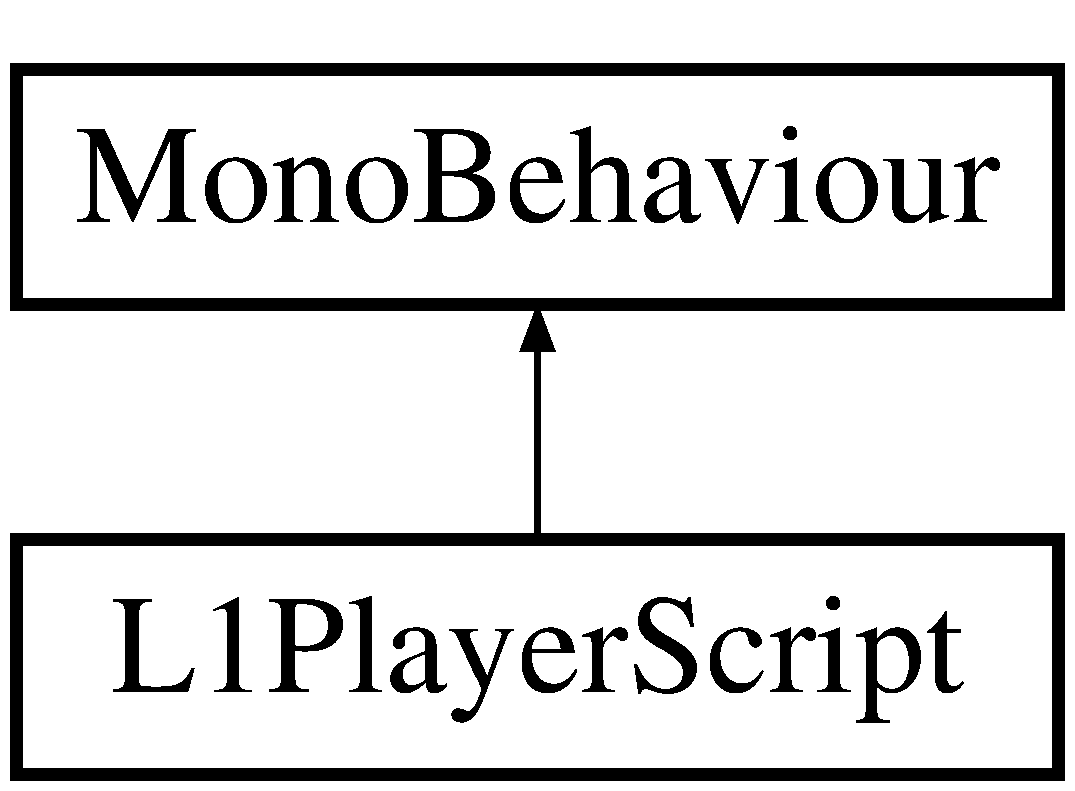
\includegraphics[height=2.000000cm]{class_l1_player_script}
\end{center}
\end{figure}
\subsection*{Public Attributes}
\begin{DoxyCompactItemize}
\item 
Audio\-Clip \hyperlink{class_l1_player_script_a8de3ae6c3ec4bc6e6df11cb70ce2a23a}{Engine\-Part}
\item 
Audio\-Clip \hyperlink{class_l1_player_script_a16ab44f36ede46fcee2935528bf69fde}{Found\-Key}
\item 
Game\-Object \hyperlink{class_l1_player_script_abe4e76e0f60f25ca1301c7bf73b10afe}{fading\-Message\-Prefab}
\item 
string \hyperlink{class_l1_player_script_afbc69f415412daadff795372b4336ab9}{engine\-Part} = \char`\"{}(message to appear)\char`\"{}
\item 
string \hyperlink{class_l1_player_script_ac3f3f18561f2bea066a3b06f84e993ea}{key\-Found} = \char`\"{}(message to appear)\char`\"{}
\end{DoxyCompactItemize}


\subsection{Detailed Description}
Class that controls the \hyperlink{class_player}{Player} on level 1. 

\begin{DoxyAuthor}{Author}
David Kelly 
\end{DoxyAuthor}
\begin{DoxyVersion}{Version}
1.\-0 
\end{DoxyVersion}
\begin{DoxyDate}{Date}
20/4/14
\end{DoxyDate}
\begin{DoxyRefDesc}{Bug}
\item[\hyperlink{bug__bug000002}{Bug}]audio is cut off when level 2 is loaded \end{DoxyRefDesc}


\subsection{Member Data Documentation}
\hypertarget{class_l1_player_script_a8de3ae6c3ec4bc6e6df11cb70ce2a23a}{\index{L1\-Player\-Script@{L1\-Player\-Script}!Engine\-Part@{Engine\-Part}}
\index{Engine\-Part@{Engine\-Part}!L1PlayerScript@{L1\-Player\-Script}}
\subsubsection[{Engine\-Part}]{\setlength{\rightskip}{0pt plus 5cm}Audio\-Clip L1\-Player\-Script.\-Engine\-Part}}\label{class_l1_player_script_a8de3ae6c3ec4bc6e6df11cb70ce2a23a}
Reference to an audio source that will play when an engine part is collided with \hypertarget{class_l1_player_script_afbc69f415412daadff795372b4336ab9}{\index{L1\-Player\-Script@{L1\-Player\-Script}!engine\-Part@{engine\-Part}}
\index{engine\-Part@{engine\-Part}!L1PlayerScript@{L1\-Player\-Script}}
\subsubsection[{engine\-Part}]{\setlength{\rightskip}{0pt plus 5cm}string L1\-Player\-Script.\-engine\-Part = \char`\"{}(message to appear)\char`\"{}}}\label{class_l1_player_script_afbc69f415412daadff795372b4336ab9}
Reference to the message entered \hypertarget{class_l1_player_script_abe4e76e0f60f25ca1301c7bf73b10afe}{\index{L1\-Player\-Script@{L1\-Player\-Script}!fading\-Message\-Prefab@{fading\-Message\-Prefab}}
\index{fading\-Message\-Prefab@{fading\-Message\-Prefab}!L1PlayerScript@{L1\-Player\-Script}}
\subsubsection[{fading\-Message\-Prefab}]{\setlength{\rightskip}{0pt plus 5cm}Game\-Object L1\-Player\-Script.\-fading\-Message\-Prefab}}\label{class_l1_player_script_abe4e76e0f60f25ca1301c7bf73b10afe}
Creating a message prefab reference \hypertarget{class_l1_player_script_a16ab44f36ede46fcee2935528bf69fde}{\index{L1\-Player\-Script@{L1\-Player\-Script}!Found\-Key@{Found\-Key}}
\index{Found\-Key@{Found\-Key}!L1PlayerScript@{L1\-Player\-Script}}
\subsubsection[{Found\-Key}]{\setlength{\rightskip}{0pt plus 5cm}Audio\-Clip L1\-Player\-Script.\-Found\-Key}}\label{class_l1_player_script_a16ab44f36ede46fcee2935528bf69fde}
Reference to an audio source that will play when an engine part is collided with \hypertarget{class_l1_player_script_ac3f3f18561f2bea066a3b06f84e993ea}{\index{L1\-Player\-Script@{L1\-Player\-Script}!key\-Found@{key\-Found}}
\index{key\-Found@{key\-Found}!L1PlayerScript@{L1\-Player\-Script}}
\subsubsection[{key\-Found}]{\setlength{\rightskip}{0pt plus 5cm}string L1\-Player\-Script.\-key\-Found = \char`\"{}(message to appear)\char`\"{}}}\label{class_l1_player_script_ac3f3f18561f2bea066a3b06f84e993ea}
Reference to the message entered 

The documentation for this class was generated from the following file\-:\begin{DoxyCompactItemize}
\item 
L1\-Player\-Script.\-cs\end{DoxyCompactItemize}

\hypertarget{class_l2_player}{\section{L2\-Player Class Reference}
\label{class_l2_player}\index{L2\-Player@{L2\-Player}}
}


Class that controls the \hyperlink{class_player}{Player} on level 2.  


Inheritance diagram for L2\-Player\-:\begin{figure}[H]
\begin{center}
\leavevmode
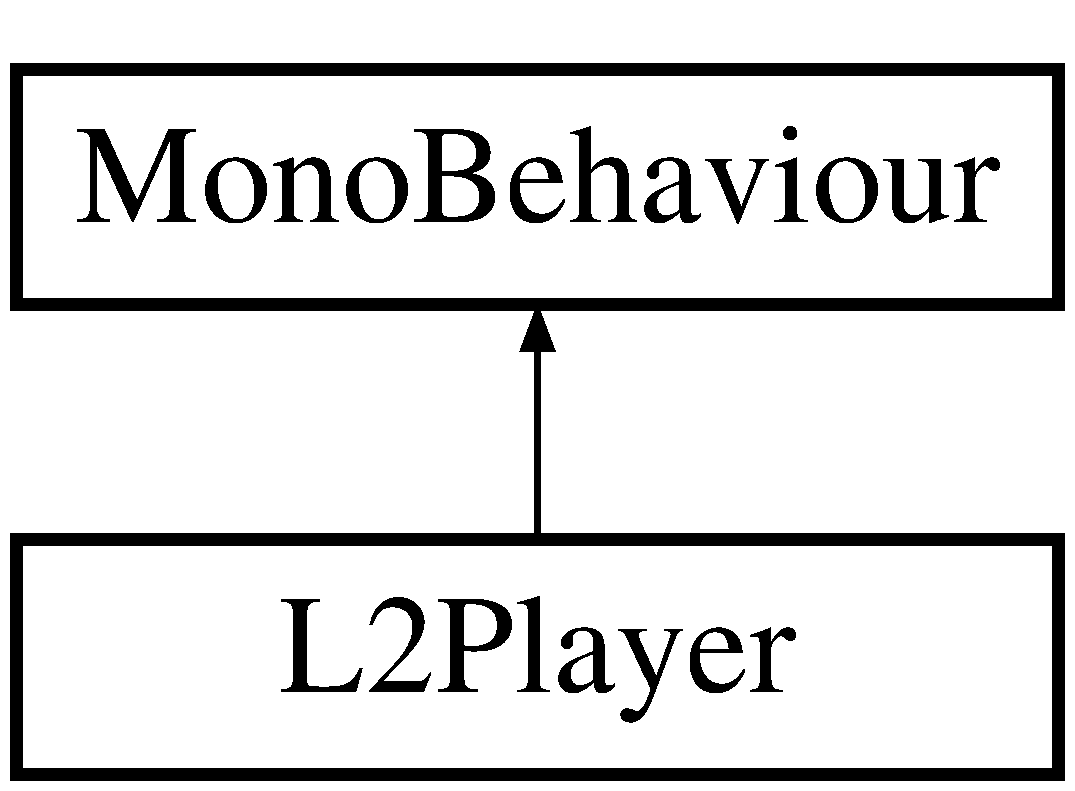
\includegraphics[height=2.000000cm]{class_l2_player}
\end{center}
\end{figure}
\subsection*{Public Member Functions}
\begin{DoxyCompactItemize}
\item 
int \hyperlink{class_l2_player_abf85322d2af4412614e90db0f177e5d7}{Get\-Parts\-Left} ()
\item 
int \hyperlink{class_l2_player_a0f061ad122d98387a8d1a5ab10a10a01}{Get\-Lives\-Left} ()
\end{DoxyCompactItemize}
\subsection*{Public Attributes}
\begin{DoxyCompactItemize}
\item 
\hypertarget{class_l2_player_ab1c41d90971c87411a23f19185c8df71}{float {\bfseries delay\-Between\-Deaths} = 0.\-5f}\label{class_l2_player_ab1c41d90971c87411a23f19185c8df71}

\item 
Audio\-Clip \hyperlink{class_l2_player_ae6acf2430aa6da4b449caa58077c1db7}{Engine\-Part}
\item 
Audio\-Clip \hyperlink{class_l2_player_a3fc2b5fdbd62fe694a1f20a6f085a43f}{Die}
\item 
Game\-Object \hyperlink{class_l2_player_ac539a32388cdac6aa327d71b6646727b}{fading\-Message\-Prefab}
\item 
string \hyperlink{class_l2_player_ac303dbde290736bcbe225855c71e3dc4}{engine\-Part} = \char`\"{}(message to appear)\char`\"{}
\item 
string \hyperlink{class_l2_player_a354ec1eb77d1e1bceac1ea9f0205dab9}{died} = \char`\"{}(message to appear)\char`\"{}
\end{DoxyCompactItemize}


\subsection{Detailed Description}
Class that controls the \hyperlink{class_player}{Player} on level 2. 

\begin{DoxyAuthor}{Author}
David Kelly 
\end{DoxyAuthor}
\begin{DoxyVersion}{Version}
1.\-0 
\end{DoxyVersion}
\begin{DoxyDate}{Date}
20/4/14 
\end{DoxyDate}


\subsection{Member Function Documentation}
\hypertarget{class_l2_player_a0f061ad122d98387a8d1a5ab10a10a01}{\index{L2\-Player@{L2\-Player}!Get\-Lives\-Left@{Get\-Lives\-Left}}
\index{Get\-Lives\-Left@{Get\-Lives\-Left}!L2Player@{L2\-Player}}
\subsubsection[{Get\-Lives\-Left}]{\setlength{\rightskip}{0pt plus 5cm}int L2\-Player.\-Get\-Lives\-Left (
\begin{DoxyParamCaption}
{}
\end{DoxyParamCaption}
)\hspace{0.3cm}{\ttfamily [inline]}}}\label{class_l2_player_a0f061ad122d98387a8d1a5ab10a10a01}
\begin{DoxyReturn}{Returns}
The number of lives the player has left in the level 
\end{DoxyReturn}
\hypertarget{class_l2_player_abf85322d2af4412614e90db0f177e5d7}{\index{L2\-Player@{L2\-Player}!Get\-Parts\-Left@{Get\-Parts\-Left}}
\index{Get\-Parts\-Left@{Get\-Parts\-Left}!L2Player@{L2\-Player}}
\subsubsection[{Get\-Parts\-Left}]{\setlength{\rightskip}{0pt plus 5cm}int L2\-Player.\-Get\-Parts\-Left (
\begin{DoxyParamCaption}
{}
\end{DoxyParamCaption}
)\hspace{0.3cm}{\ttfamily [inline]}}}\label{class_l2_player_abf85322d2af4412614e90db0f177e5d7}
\begin{DoxyReturn}{Returns}
The number of parts left to collect in the level 
\end{DoxyReturn}


\subsection{Member Data Documentation}
\hypertarget{class_l2_player_a3fc2b5fdbd62fe694a1f20a6f085a43f}{\index{L2\-Player@{L2\-Player}!Die@{Die}}
\index{Die@{Die}!L2Player@{L2\-Player}}
\subsubsection[{Die}]{\setlength{\rightskip}{0pt plus 5cm}Audio\-Clip L2\-Player.\-Die}}\label{class_l2_player_a3fc2b5fdbd62fe694a1f20a6f085a43f}
Reference to an audio source that will play when a Badguy is collided with \hypertarget{class_l2_player_a354ec1eb77d1e1bceac1ea9f0205dab9}{\index{L2\-Player@{L2\-Player}!died@{died}}
\index{died@{died}!L2Player@{L2\-Player}}
\subsubsection[{died}]{\setlength{\rightskip}{0pt plus 5cm}string L2\-Player.\-died = \char`\"{}(message to appear)\char`\"{}}}\label{class_l2_player_a354ec1eb77d1e1bceac1ea9f0205dab9}
Reference to the message entered \hypertarget{class_l2_player_ae6acf2430aa6da4b449caa58077c1db7}{\index{L2\-Player@{L2\-Player}!Engine\-Part@{Engine\-Part}}
\index{Engine\-Part@{Engine\-Part}!L2Player@{L2\-Player}}
\subsubsection[{Engine\-Part}]{\setlength{\rightskip}{0pt plus 5cm}Audio\-Clip L2\-Player.\-Engine\-Part}}\label{class_l2_player_ae6acf2430aa6da4b449caa58077c1db7}
Reference to an audio source that will play when an engine part is collided with \hypertarget{class_l2_player_ac303dbde290736bcbe225855c71e3dc4}{\index{L2\-Player@{L2\-Player}!engine\-Part@{engine\-Part}}
\index{engine\-Part@{engine\-Part}!L2Player@{L2\-Player}}
\subsubsection[{engine\-Part}]{\setlength{\rightskip}{0pt plus 5cm}string L2\-Player.\-engine\-Part = \char`\"{}(message to appear)\char`\"{}}}\label{class_l2_player_ac303dbde290736bcbe225855c71e3dc4}
Reference to the message entered \hypertarget{class_l2_player_ac539a32388cdac6aa327d71b6646727b}{\index{L2\-Player@{L2\-Player}!fading\-Message\-Prefab@{fading\-Message\-Prefab}}
\index{fading\-Message\-Prefab@{fading\-Message\-Prefab}!L2Player@{L2\-Player}}
\subsubsection[{fading\-Message\-Prefab}]{\setlength{\rightskip}{0pt plus 5cm}Game\-Object L2\-Player.\-fading\-Message\-Prefab}}\label{class_l2_player_ac539a32388cdac6aa327d71b6646727b}
Creating a message prefab reference 

The documentation for this class was generated from the following file\-:\begin{DoxyCompactItemize}
\item 
L2\-Player.\-cs\end{DoxyCompactItemize}

\hypertarget{class_l2_player_engine_icon}{\section{L2\-Player\-Engine\-Icon Class Reference}
\label{class_l2_player_engine_icon}\index{L2\-Player\-Engine\-Icon@{L2\-Player\-Engine\-Icon}}
}


Class that displays the engine icons on the screen.  


Inheritance diagram for L2\-Player\-Engine\-Icon\-:\begin{figure}[H]
\begin{center}
\leavevmode
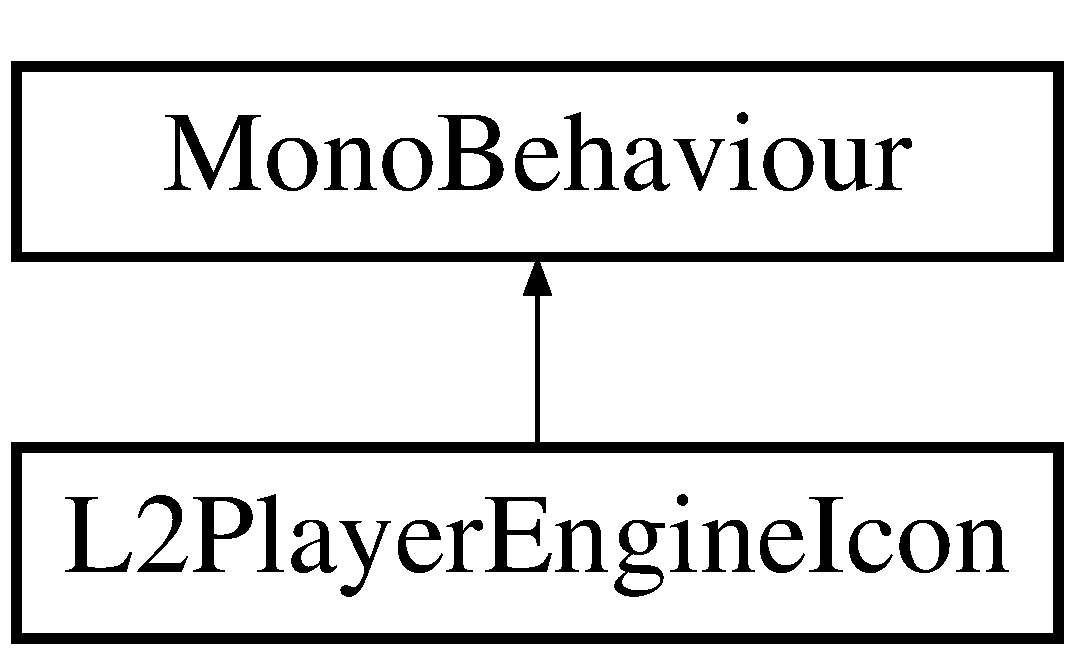
\includegraphics[height=2.000000cm]{class_l2_player_engine_icon}
\end{center}
\end{figure}
\subsection*{Public Attributes}
\begin{DoxyCompactItemize}
\item 
\hyperlink{class_l2_player}{L2\-Player} \hyperlink{class_l2_player_engine_icon_aade810346a1d59d61fe8775670926534}{player}
\item 
Texture \hyperlink{class_l2_player_engine_icon_a634b2ec6b0dfb77eca75328c43986b77}{engine\-On}
\end{DoxyCompactItemize}


\subsection{Detailed Description}
Class that displays the engine icons on the screen. 

\begin{DoxyAuthor}{Author}
David Kelly 
\end{DoxyAuthor}
\begin{DoxyVersion}{Version}
1.\-0 
\end{DoxyVersion}
\begin{DoxyDate}{Date}
20/4/14 
\end{DoxyDate}


\subsection{Member Data Documentation}
\hypertarget{class_l2_player_engine_icon_a634b2ec6b0dfb77eca75328c43986b77}{\index{L2\-Player\-Engine\-Icon@{L2\-Player\-Engine\-Icon}!engine\-On@{engine\-On}}
\index{engine\-On@{engine\-On}!L2PlayerEngineIcon@{L2\-Player\-Engine\-Icon}}
\subsubsection[{engine\-On}]{\setlength{\rightskip}{0pt plus 5cm}Texture L2\-Player\-Engine\-Icon.\-engine\-On}}\label{class_l2_player_engine_icon_a634b2ec6b0dfb77eca75328c43986b77}
Reference to the image displayed on the screen representing the engine parts \hypertarget{class_l2_player_engine_icon_aade810346a1d59d61fe8775670926534}{\index{L2\-Player\-Engine\-Icon@{L2\-Player\-Engine\-Icon}!player@{player}}
\index{player@{player}!L2PlayerEngineIcon@{L2\-Player\-Engine\-Icon}}
\subsubsection[{player}]{\setlength{\rightskip}{0pt plus 5cm}{\bf L2\-Player} L2\-Player\-Engine\-Icon.\-player}}\label{class_l2_player_engine_icon_aade810346a1d59d61fe8775670926534}
Reference to the player collecting the engine parts 

The documentation for this class was generated from the following file\-:\begin{DoxyCompactItemize}
\item 
L2\-Player\-Engine\-Icon.\-cs\end{DoxyCompactItemize}

\hypertarget{class_l2_player_g_u_i}{\section{L2\-Player\-G\-U\-I Class Reference}
\label{class_l2_player_g_u_i}\index{L2\-Player\-G\-U\-I@{L2\-Player\-G\-U\-I}}
}


Class that displays the players lives left on level 2.  


Inheritance diagram for L2\-Player\-G\-U\-I\-:\begin{figure}[H]
\begin{center}
\leavevmode
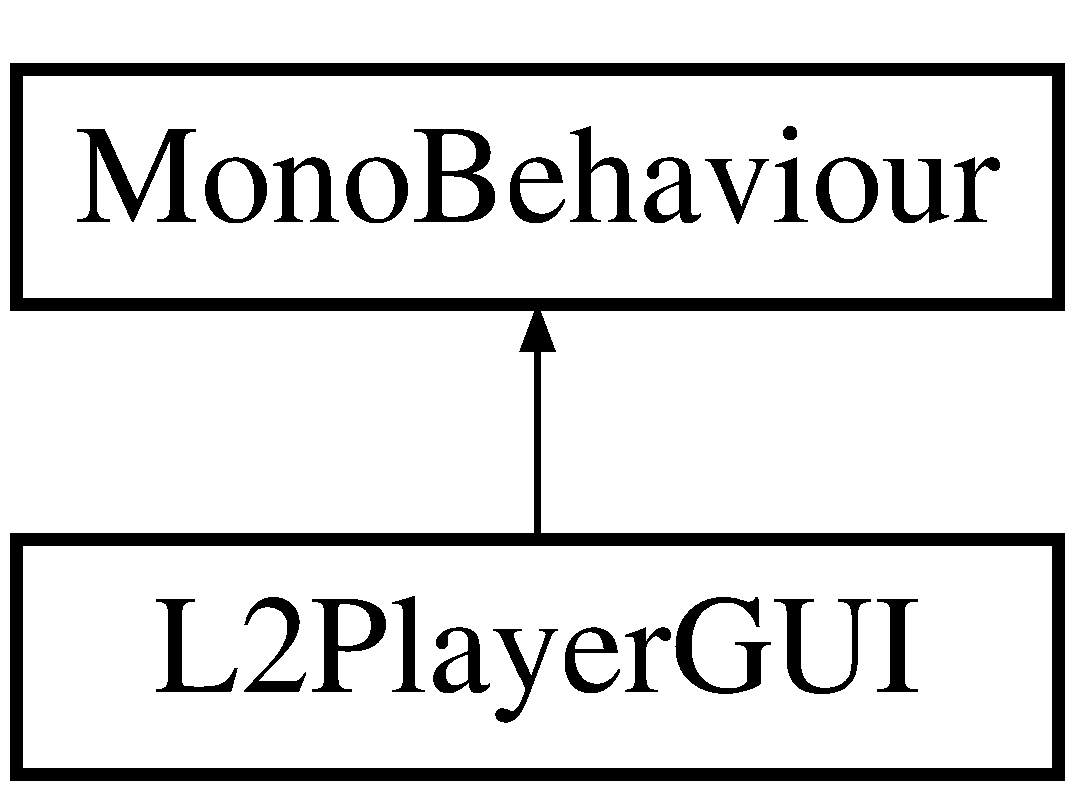
\includegraphics[height=2.000000cm]{class_l2_player_g_u_i}
\end{center}
\end{figure}
\subsection*{Public Attributes}
\begin{DoxyCompactItemize}
\item 
\hyperlink{class_l2_player}{L2\-Player} \hyperlink{class_l2_player_g_u_i_abafb0f674da5f4bae17845439ef20140}{player}
\item 
Texture \hyperlink{class_l2_player_g_u_i_a9e2d8835c594cbc9521849c35ddde0dc}{robot\-Life}
\end{DoxyCompactItemize}


\subsection{Detailed Description}
Class that displays the players lives left on level 2. 

\begin{DoxyAuthor}{Author}
David Kelly 
\end{DoxyAuthor}
\begin{DoxyVersion}{Version}
1.\-0 
\end{DoxyVersion}
\begin{DoxyDate}{Date}
20/4/14 
\end{DoxyDate}


\subsection{Member Data Documentation}
\hypertarget{class_l2_player_g_u_i_abafb0f674da5f4bae17845439ef20140}{\index{L2\-Player\-G\-U\-I@{L2\-Player\-G\-U\-I}!player@{player}}
\index{player@{player}!L2PlayerGUI@{L2\-Player\-G\-U\-I}}
\subsubsection[{player}]{\setlength{\rightskip}{0pt plus 5cm}{\bf L2\-Player} L2\-Player\-G\-U\-I.\-player}}\label{class_l2_player_g_u_i_abafb0f674da5f4bae17845439ef20140}
Reference to the player object the lives are related to \hypertarget{class_l2_player_g_u_i_a9e2d8835c594cbc9521849c35ddde0dc}{\index{L2\-Player\-G\-U\-I@{L2\-Player\-G\-U\-I}!robot\-Life@{robot\-Life}}
\index{robot\-Life@{robot\-Life}!L2PlayerGUI@{L2\-Player\-G\-U\-I}}
\subsubsection[{robot\-Life}]{\setlength{\rightskip}{0pt plus 5cm}Texture L2\-Player\-G\-U\-I.\-robot\-Life}}\label{class_l2_player_g_u_i_a9e2d8835c594cbc9521849c35ddde0dc}
Reference to the image used to represent the lives 

The documentation for this class was generated from the following file\-:\begin{DoxyCompactItemize}
\item 
L2\-Player\-G\-U\-I.\-cs\end{DoxyCompactItemize}

\hypertarget{class_l2_ship_sensor}{\section{L2\-Ship\-Sensor Class Reference}
\label{class_l2_ship_sensor}\index{L2\-Ship\-Sensor@{L2\-Ship\-Sensor}}
}


Controls whether the player collected all the parts needed to fix the ship when trigger is entered.  


Inheritance diagram for L2\-Ship\-Sensor\-:\begin{figure}[H]
\begin{center}
\leavevmode
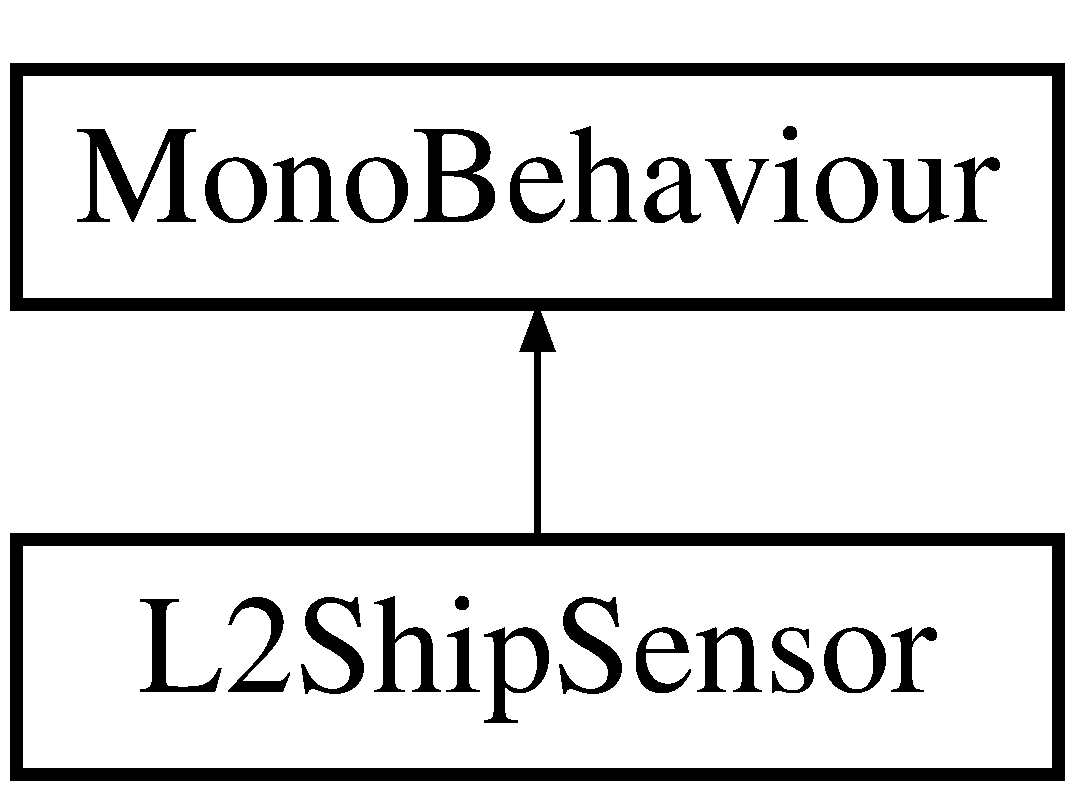
\includegraphics[height=2.000000cm]{class_l2_ship_sensor}
\end{center}
\end{figure}
\subsection*{Public Attributes}
\begin{DoxyCompactItemize}
\item 
Game\-Object \hyperlink{class_l2_ship_sensor_a116a957e82ee35d2680cafd6d2dd53c0}{ship\-G\-O}
\item 
Audio\-Clip \hyperlink{class_l2_ship_sensor_a92c76b2b502112bc9c298154f77c76b1}{ship\-Start}
\item 
Game\-Object \hyperlink{class_l2_ship_sensor_a2d8958af9884c632331a9e031b9cfc78}{fading\-Message\-Prefab}
\item 
string \hyperlink{class_l2_ship_sensor_ab0ce9e2c72170c03532ad0f45ab105c1}{get\-Parts} = \char`\"{}(message to appear)\char`\"{}
\item 
string \hyperlink{class_l2_ship_sensor_aa262461caa8e7f1eaa5e65cc949cd16b}{complete} = \char`\"{}(message to appear)\char`\"{}
\end{DoxyCompactItemize}


\subsection{Detailed Description}
Controls whether the player collected all the parts needed to fix the ship when trigger is entered. 

\begin{DoxyAuthor}{Author}
David Kelly 
\end{DoxyAuthor}
\begin{DoxyVersion}{Version}
1.\-0 
\end{DoxyVersion}
\begin{DoxyDate}{Date}
20/4/14
\end{DoxyDate}
\begin{DoxyWarning}{Warning}
return values for engine parts needed from the player game object
\end{DoxyWarning}
\begin{DoxyRefDesc}{Bug}
\item[\hyperlink{bug__bug000003}{Bug}]audio is skipped when game level is loaded \end{DoxyRefDesc}


\subsection{Member Data Documentation}
\hypertarget{class_l2_ship_sensor_aa262461caa8e7f1eaa5e65cc949cd16b}{\index{L2\-Ship\-Sensor@{L2\-Ship\-Sensor}!complete@{complete}}
\index{complete@{complete}!L2ShipSensor@{L2\-Ship\-Sensor}}
\subsubsection[{complete}]{\setlength{\rightskip}{0pt plus 5cm}string L2\-Ship\-Sensor.\-complete = \char`\"{}(message to appear)\char`\"{}}}\label{class_l2_ship_sensor_aa262461caa8e7f1eaa5e65cc949cd16b}
Reference to the message entered \hypertarget{class_l2_ship_sensor_a2d8958af9884c632331a9e031b9cfc78}{\index{L2\-Ship\-Sensor@{L2\-Ship\-Sensor}!fading\-Message\-Prefab@{fading\-Message\-Prefab}}
\index{fading\-Message\-Prefab@{fading\-Message\-Prefab}!L2ShipSensor@{L2\-Ship\-Sensor}}
\subsubsection[{fading\-Message\-Prefab}]{\setlength{\rightskip}{0pt plus 5cm}Game\-Object L2\-Ship\-Sensor.\-fading\-Message\-Prefab}}\label{class_l2_ship_sensor_a2d8958af9884c632331a9e031b9cfc78}
Reference to the fading message game object \hypertarget{class_l2_ship_sensor_ab0ce9e2c72170c03532ad0f45ab105c1}{\index{L2\-Ship\-Sensor@{L2\-Ship\-Sensor}!get\-Parts@{get\-Parts}}
\index{get\-Parts@{get\-Parts}!L2ShipSensor@{L2\-Ship\-Sensor}}
\subsubsection[{get\-Parts}]{\setlength{\rightskip}{0pt plus 5cm}string L2\-Ship\-Sensor.\-get\-Parts = \char`\"{}(message to appear)\char`\"{}}}\label{class_l2_ship_sensor_ab0ce9e2c72170c03532ad0f45ab105c1}
Reference to the message entered \hypertarget{class_l2_ship_sensor_a116a957e82ee35d2680cafd6d2dd53c0}{\index{L2\-Ship\-Sensor@{L2\-Ship\-Sensor}!ship\-G\-O@{ship\-G\-O}}
\index{ship\-G\-O@{ship\-G\-O}!L2ShipSensor@{L2\-Ship\-Sensor}}
\subsubsection[{ship\-G\-O}]{\setlength{\rightskip}{0pt plus 5cm}Game\-Object L2\-Ship\-Sensor.\-ship\-G\-O}}\label{class_l2_ship_sensor_a116a957e82ee35d2680cafd6d2dd53c0}
Reference to the ship game object \hypertarget{class_l2_ship_sensor_a92c76b2b502112bc9c298154f77c76b1}{\index{L2\-Ship\-Sensor@{L2\-Ship\-Sensor}!ship\-Start@{ship\-Start}}
\index{ship\-Start@{ship\-Start}!L2ShipSensor@{L2\-Ship\-Sensor}}
\subsubsection[{ship\-Start}]{\setlength{\rightskip}{0pt plus 5cm}Audio\-Clip L2\-Ship\-Sensor.\-ship\-Start}}\label{class_l2_ship_sensor_a92c76b2b502112bc9c298154f77c76b1}
Reference to the audio file 

The documentation for this class was generated from the following file\-:\begin{DoxyCompactItemize}
\item 
L2\-Ship\-Sensor.\-cs\end{DoxyCompactItemize}

\hypertarget{class_player}{\section{Player Class Reference}
\label{class_player}\index{Player@{Player}}
}


Class that controls the player for level 3.  


Inheritance diagram for Player\-:\begin{figure}[H]
\begin{center}
\leavevmode
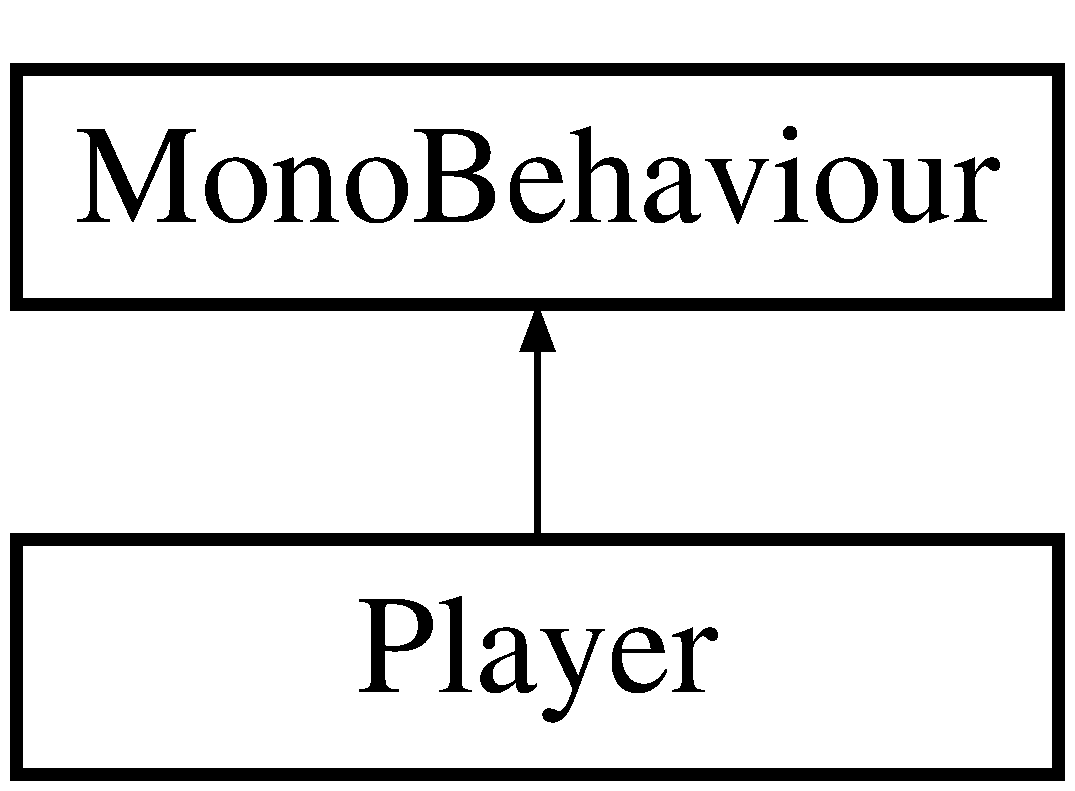
\includegraphics[height=2.000000cm]{class_player}
\end{center}
\end{figure}
\subsection*{Public Member Functions}
\begin{DoxyCompactItemize}
\item 
int \hyperlink{class_player_aed4d068363ffab322450dec4b674b43c}{Get\-Parts\-Left} ()
\item 
int \hyperlink{class_player_a35c51977648cc3b95a7074839a6f651a}{Get\-Lives\-Left} ()
\item 
int \hyperlink{class_player_afee1105ef952044bf9841cdaa199af0d}{Get\-Key\-Count} ()
\item 
bool \hyperlink{class_player_aa186cee2b963a62fd691f6e8f98e17ae}{Is\-Carrying\-Key} ()
\item 
void \hyperlink{class_player_a961fc1484a835f436ea9db34cd5dba7d}{Drop\-Key} ()
\end{DoxyCompactItemize}
\subsection*{Public Attributes}
\begin{DoxyCompactItemize}
\item 
\hypertarget{class_player_a690ec1561aafce0f3e480de83c707261}{float {\bfseries delay\-Between\-Deaths} = 0.\-5f}\label{class_player_a690ec1561aafce0f3e480de83c707261}

\item 
Audio\-Clip \hyperlink{class_player_afbe782b06cf141675680af069408cd6a}{Engine\-Part}
\item 
Audio\-Clip \hyperlink{class_player_a8e34fba594dbf68174d883d763d42ace}{Die}
\item 
Audio\-Clip \hyperlink{class_player_ae0ed5e4ea70a02e3f9c0ee8964c4fd64}{Found\-Key}
\item 
Game\-Object \hyperlink{class_player_a13d88e1c4562fddf90baf0d57afc68c5}{fading\-Message\-Prefab}
\item 
string \hyperlink{class_player_a66e422e9d0486bdb42c835142caa93c6}{engine\-Part} = \char`\"{}(message to appear)\char`\"{}
\item 
string \hyperlink{class_player_a998c3019f31ab3ad606453158abe9dcb}{died} = \char`\"{}(message to appear)\char`\"{}
\end{DoxyCompactItemize}


\subsection{Detailed Description}
Class that controls the player for level 3. 

\begin{DoxyAuthor}{Author}
David Kelly 
\end{DoxyAuthor}
\begin{DoxyVersion}{Version}
1.\-0 
\end{DoxyVersion}
\begin{DoxyDate}{Date}
20/4/14
\end{DoxyDate}
\begin{DoxyRefDesc}{Bug}
\item[\hyperlink{bug__bug000004}{Bug}]if player loses all his lives the audio is interrupted by the new level loaded \end{DoxyRefDesc}


\subsection{Member Function Documentation}
\hypertarget{class_player_a961fc1484a835f436ea9db34cd5dba7d}{\index{Player@{Player}!Drop\-Key@{Drop\-Key}}
\index{Drop\-Key@{Drop\-Key}!Player@{Player}}
\subsubsection[{Drop\-Key}]{\setlength{\rightskip}{0pt plus 5cm}void Player.\-Drop\-Key (
\begin{DoxyParamCaption}
{}
\end{DoxyParamCaption}
)\hspace{0.3cm}{\ttfamily [inline]}}}\label{class_player_a961fc1484a835f436ea9db34cd5dba7d}
Method that removes the key item for the player after opening the door \hypertarget{class_player_afee1105ef952044bf9841cdaa199af0d}{\index{Player@{Player}!Get\-Key\-Count@{Get\-Key\-Count}}
\index{Get\-Key\-Count@{Get\-Key\-Count}!Player@{Player}}
\subsubsection[{Get\-Key\-Count}]{\setlength{\rightskip}{0pt plus 5cm}int Player.\-Get\-Key\-Count (
\begin{DoxyParamCaption}
{}
\end{DoxyParamCaption}
)\hspace{0.3cm}{\ttfamily [inline]}}}\label{class_player_afee1105ef952044bf9841cdaa199af0d}
Method that returns the integer value of the key left in level 3 \begin{DoxyReturn}{Returns}
integer value 
\end{DoxyReturn}
\hypertarget{class_player_a35c51977648cc3b95a7074839a6f651a}{\index{Player@{Player}!Get\-Lives\-Left@{Get\-Lives\-Left}}
\index{Get\-Lives\-Left@{Get\-Lives\-Left}!Player@{Player}}
\subsubsection[{Get\-Lives\-Left}]{\setlength{\rightskip}{0pt plus 5cm}int Player.\-Get\-Lives\-Left (
\begin{DoxyParamCaption}
{}
\end{DoxyParamCaption}
)\hspace{0.3cm}{\ttfamily [inline]}}}\label{class_player_a35c51977648cc3b95a7074839a6f651a}
\begin{DoxyReturn}{Returns}
Returns the lives remaining for the player on level 3 
\end{DoxyReturn}
\hypertarget{class_player_aed4d068363ffab322450dec4b674b43c}{\index{Player@{Player}!Get\-Parts\-Left@{Get\-Parts\-Left}}
\index{Get\-Parts\-Left@{Get\-Parts\-Left}!Player@{Player}}
\subsubsection[{Get\-Parts\-Left}]{\setlength{\rightskip}{0pt plus 5cm}int Player.\-Get\-Parts\-Left (
\begin{DoxyParamCaption}
{}
\end{DoxyParamCaption}
)\hspace{0.3cm}{\ttfamily [inline]}}}\label{class_player_aed4d068363ffab322450dec4b674b43c}
\begin{DoxyReturn}{Returns}
Returns the int value of the remaining Engine Parts on level 3 
\end{DoxyReturn}
\hypertarget{class_player_aa186cee2b963a62fd691f6e8f98e17ae}{\index{Player@{Player}!Is\-Carrying\-Key@{Is\-Carrying\-Key}}
\index{Is\-Carrying\-Key@{Is\-Carrying\-Key}!Player@{Player}}
\subsubsection[{Is\-Carrying\-Key}]{\setlength{\rightskip}{0pt plus 5cm}bool Player.\-Is\-Carrying\-Key (
\begin{DoxyParamCaption}
{}
\end{DoxyParamCaption}
)\hspace{0.3cm}{\ttfamily [inline]}}}\label{class_player_aa186cee2b963a62fd691f6e8f98e17ae}
Method that returns the boolean value reference to if the player has the key \begin{DoxyReturn}{Returns}
boolean value 
\end{DoxyReturn}


\subsection{Member Data Documentation}
\hypertarget{class_player_a8e34fba594dbf68174d883d763d42ace}{\index{Player@{Player}!Die@{Die}}
\index{Die@{Die}!Player@{Player}}
\subsubsection[{Die}]{\setlength{\rightskip}{0pt plus 5cm}Audio\-Clip Player.\-Die}}\label{class_player_a8e34fba594dbf68174d883d763d42ace}
Reference to the audio clip file \hypertarget{class_player_a998c3019f31ab3ad606453158abe9dcb}{\index{Player@{Player}!died@{died}}
\index{died@{died}!Player@{Player}}
\subsubsection[{died}]{\setlength{\rightskip}{0pt plus 5cm}string Player.\-died = \char`\"{}(message to appear)\char`\"{}}}\label{class_player_a998c3019f31ab3ad606453158abe9dcb}
Reference to the message that will appear \hypertarget{class_player_afbe782b06cf141675680af069408cd6a}{\index{Player@{Player}!Engine\-Part@{Engine\-Part}}
\index{Engine\-Part@{Engine\-Part}!Player@{Player}}
\subsubsection[{Engine\-Part}]{\setlength{\rightskip}{0pt plus 5cm}Audio\-Clip Player.\-Engine\-Part}}\label{class_player_afbe782b06cf141675680af069408cd6a}
Reference to the audio clip file \hypertarget{class_player_a66e422e9d0486bdb42c835142caa93c6}{\index{Player@{Player}!engine\-Part@{engine\-Part}}
\index{engine\-Part@{engine\-Part}!Player@{Player}}
\subsubsection[{engine\-Part}]{\setlength{\rightskip}{0pt plus 5cm}string Player.\-engine\-Part = \char`\"{}(message to appear)\char`\"{}}}\label{class_player_a66e422e9d0486bdb42c835142caa93c6}
Reference to the message that will appear \hypertarget{class_player_a13d88e1c4562fddf90baf0d57afc68c5}{\index{Player@{Player}!fading\-Message\-Prefab@{fading\-Message\-Prefab}}
\index{fading\-Message\-Prefab@{fading\-Message\-Prefab}!Player@{Player}}
\subsubsection[{fading\-Message\-Prefab}]{\setlength{\rightskip}{0pt plus 5cm}Game\-Object Player.\-fading\-Message\-Prefab}}\label{class_player_a13d88e1c4562fddf90baf0d57afc68c5}
Creating a message prefab reference \hypertarget{class_player_ae0ed5e4ea70a02e3f9c0ee8964c4fd64}{\index{Player@{Player}!Found\-Key@{Found\-Key}}
\index{Found\-Key@{Found\-Key}!Player@{Player}}
\subsubsection[{Found\-Key}]{\setlength{\rightskip}{0pt plus 5cm}Audio\-Clip Player.\-Found\-Key}}\label{class_player_ae0ed5e4ea70a02e3f9c0ee8964c4fd64}
Reference to the audio clip file 

The documentation for this class was generated from the following file\-:\begin{DoxyCompactItemize}
\item 
Player.\-cs\end{DoxyCompactItemize}

\hypertarget{class_player_engine_icon}{\section{Player\-Engine\-Icon Class Reference}
\label{class_player_engine_icon}\index{Player\-Engine\-Icon@{Player\-Engine\-Icon}}
}


Class that displays the engine icons on the screen.  


Inheritance diagram for Player\-Engine\-Icon\-:\begin{figure}[H]
\begin{center}
\leavevmode
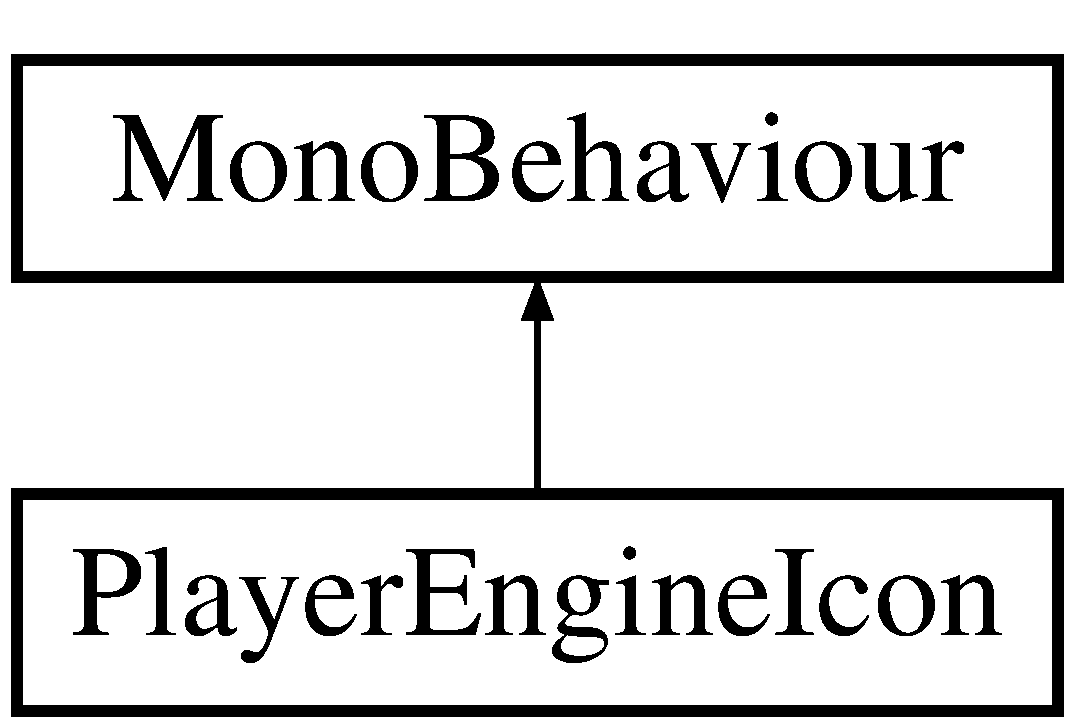
\includegraphics[height=2.000000cm]{class_player_engine_icon}
\end{center}
\end{figure}
\subsection*{Public Attributes}
\begin{DoxyCompactItemize}
\item 
\hyperlink{class_player}{Player} \hyperlink{class_player_engine_icon_aa4786c7c7622809d7361e6a35dfac6c5}{player}
\item 
Texture \hyperlink{class_player_engine_icon_aa98ba90a581a22a8a13527076251325c}{engine\-On}
\end{DoxyCompactItemize}


\subsection{Detailed Description}
Class that displays the engine icons on the screen. 

\begin{DoxyAuthor}{Author}
David Kelly 
\end{DoxyAuthor}
\begin{DoxyVersion}{Version}
1.\-0 
\end{DoxyVersion}
\begin{DoxyDate}{Date}
20/4/14 
\end{DoxyDate}


\subsection{Member Data Documentation}
\hypertarget{class_player_engine_icon_aa98ba90a581a22a8a13527076251325c}{\index{Player\-Engine\-Icon@{Player\-Engine\-Icon}!engine\-On@{engine\-On}}
\index{engine\-On@{engine\-On}!PlayerEngineIcon@{Player\-Engine\-Icon}}
\subsubsection[{engine\-On}]{\setlength{\rightskip}{0pt plus 5cm}Texture Player\-Engine\-Icon.\-engine\-On}}\label{class_player_engine_icon_aa98ba90a581a22a8a13527076251325c}
Reference to the image displayed on the screen representing the engine parts \hypertarget{class_player_engine_icon_aa4786c7c7622809d7361e6a35dfac6c5}{\index{Player\-Engine\-Icon@{Player\-Engine\-Icon}!player@{player}}
\index{player@{player}!PlayerEngineIcon@{Player\-Engine\-Icon}}
\subsubsection[{player}]{\setlength{\rightskip}{0pt plus 5cm}{\bf Player} Player\-Engine\-Icon.\-player}}\label{class_player_engine_icon_aa4786c7c7622809d7361e6a35dfac6c5}
Reference to the player collecting the engine parts 

The documentation for this class was generated from the following file\-:\begin{DoxyCompactItemize}
\item 
Player\-Engine\-Icon.\-cs\end{DoxyCompactItemize}

\hypertarget{class_player_g_u_i}{\section{Player\-G\-U\-I Class Reference}
\label{class_player_g_u_i}\index{Player\-G\-U\-I@{Player\-G\-U\-I}}
}


Class that displays the players lives left on level 3.  


Inheritance diagram for Player\-G\-U\-I\-:\begin{figure}[H]
\begin{center}
\leavevmode
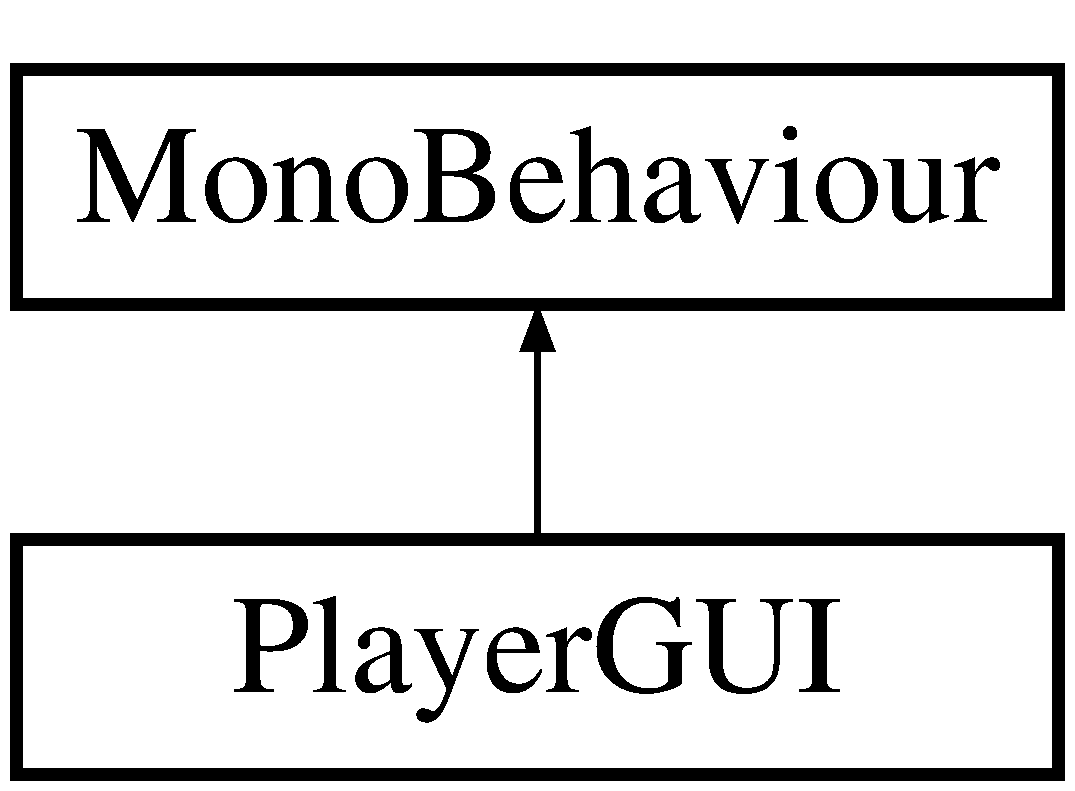
\includegraphics[height=2.000000cm]{class_player_g_u_i}
\end{center}
\end{figure}
\subsection*{Public Attributes}
\begin{DoxyCompactItemize}
\item 
\hyperlink{class_player}{Player} \hyperlink{class_player_g_u_i_a40c0f7c540fc730e1991db977edbcfb4}{player}
\item 
Texture \hyperlink{class_player_g_u_i_a71b0c8060bfd05c34d73ff6f271fd24b}{robot\-Life}
\end{DoxyCompactItemize}


\subsection{Detailed Description}
Class that displays the players lives left on level 3. 

\begin{DoxyAuthor}{Author}
David Kelly 
\end{DoxyAuthor}
\begin{DoxyVersion}{Version}
1.\-0 
\end{DoxyVersion}
\begin{DoxyDate}{Date}
20/4/14 
\end{DoxyDate}


\subsection{Member Data Documentation}
\hypertarget{class_player_g_u_i_a40c0f7c540fc730e1991db977edbcfb4}{\index{Player\-G\-U\-I@{Player\-G\-U\-I}!player@{player}}
\index{player@{player}!PlayerGUI@{Player\-G\-U\-I}}
\subsubsection[{player}]{\setlength{\rightskip}{0pt plus 5cm}{\bf Player} Player\-G\-U\-I.\-player}}\label{class_player_g_u_i_a40c0f7c540fc730e1991db977edbcfb4}
Reference to the player object the lives are related to \hypertarget{class_player_g_u_i_a71b0c8060bfd05c34d73ff6f271fd24b}{\index{Player\-G\-U\-I@{Player\-G\-U\-I}!robot\-Life@{robot\-Life}}
\index{robot\-Life@{robot\-Life}!PlayerGUI@{Player\-G\-U\-I}}
\subsubsection[{robot\-Life}]{\setlength{\rightskip}{0pt plus 5cm}Texture Player\-G\-U\-I.\-robot\-Life}}\label{class_player_g_u_i_a71b0c8060bfd05c34d73ff6f271fd24b}
Reference to the image used to represent the lives 

The documentation for this class was generated from the following file\-:\begin{DoxyCompactItemize}
\item 
Player\-G\-U\-I.\-cs\end{DoxyCompactItemize}

\hypertarget{class_player_inventory_icon}{\section{Player\-Inventory\-Icon Class Reference}
\label{class_player_inventory_icon}\index{Player\-Inventory\-Icon@{Player\-Inventory\-Icon}}
}


Class that manages the display of the key icon if the player has the key or not.  


Inheritance diagram for Player\-Inventory\-Icon\-:\begin{figure}[H]
\begin{center}
\leavevmode
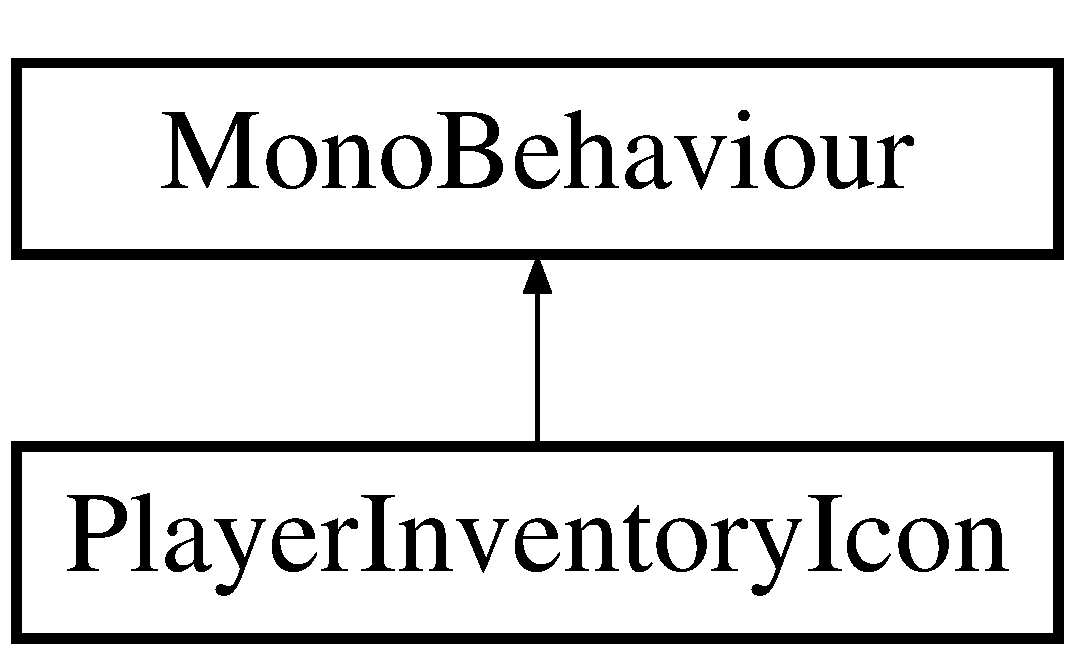
\includegraphics[height=2.000000cm]{class_player_inventory_icon}
\end{center}
\end{figure}
\subsection*{Public Attributes}
\begin{DoxyCompactItemize}
\item 
\hyperlink{class_player}{Player} \hyperlink{class_player_inventory_icon_af275fab92eb9bacfad048d1506dbd128}{player}
\item 
Texture \hyperlink{class_player_inventory_icon_a77a36854eb69ad8e1065b3020389cde0}{key\-Icon}
\item 
Texture \hyperlink{class_player_inventory_icon_adc17dc396f9f6cc8f57ecad911b68485}{empty\-Icon}
\item 
Game\-Object \hyperlink{class_player_inventory_icon_a860fe9f495c97467135ca7eaf51211d9}{fading\-Message\-Prefab}
\item 
string \hyperlink{class_player_inventory_icon_a1cfc870c87a3efae9dd66089cadc0485}{message\-Text} = \char`\"{}(message to appear)\char`\"{}
\end{DoxyCompactItemize}


\subsection{Detailed Description}
Class that manages the display of the key icon if the player has the key or not. 

\begin{DoxyAuthor}{Author}
David Kelly 
\end{DoxyAuthor}
\begin{DoxyVersion}{Version}
1.\-0 
\end{DoxyVersion}
\begin{DoxyDate}{Date}
20/4/14 
\end{DoxyDate}


\subsection{Member Data Documentation}
\hypertarget{class_player_inventory_icon_adc17dc396f9f6cc8f57ecad911b68485}{\index{Player\-Inventory\-Icon@{Player\-Inventory\-Icon}!empty\-Icon@{empty\-Icon}}
\index{empty\-Icon@{empty\-Icon}!PlayerInventoryIcon@{Player\-Inventory\-Icon}}
\subsubsection[{empty\-Icon}]{\setlength{\rightskip}{0pt plus 5cm}Texture Player\-Inventory\-Icon.\-empty\-Icon}}\label{class_player_inventory_icon_adc17dc396f9f6cc8f57ecad911b68485}
Reference to the image file \hypertarget{class_player_inventory_icon_a860fe9f495c97467135ca7eaf51211d9}{\index{Player\-Inventory\-Icon@{Player\-Inventory\-Icon}!fading\-Message\-Prefab@{fading\-Message\-Prefab}}
\index{fading\-Message\-Prefab@{fading\-Message\-Prefab}!PlayerInventoryIcon@{Player\-Inventory\-Icon}}
\subsubsection[{fading\-Message\-Prefab}]{\setlength{\rightskip}{0pt plus 5cm}Game\-Object Player\-Inventory\-Icon.\-fading\-Message\-Prefab}}\label{class_player_inventory_icon_a860fe9f495c97467135ca7eaf51211d9}
Reference to the fading message prefab \hypertarget{class_player_inventory_icon_a77a36854eb69ad8e1065b3020389cde0}{\index{Player\-Inventory\-Icon@{Player\-Inventory\-Icon}!key\-Icon@{key\-Icon}}
\index{key\-Icon@{key\-Icon}!PlayerInventoryIcon@{Player\-Inventory\-Icon}}
\subsubsection[{key\-Icon}]{\setlength{\rightskip}{0pt plus 5cm}Texture Player\-Inventory\-Icon.\-key\-Icon}}\label{class_player_inventory_icon_a77a36854eb69ad8e1065b3020389cde0}
Reference to the image file \hypertarget{class_player_inventory_icon_a1cfc870c87a3efae9dd66089cadc0485}{\index{Player\-Inventory\-Icon@{Player\-Inventory\-Icon}!message\-Text@{message\-Text}}
\index{message\-Text@{message\-Text}!PlayerInventoryIcon@{Player\-Inventory\-Icon}}
\subsubsection[{message\-Text}]{\setlength{\rightskip}{0pt plus 5cm}string Player\-Inventory\-Icon.\-message\-Text = \char`\"{}(message to appear)\char`\"{}}}\label{class_player_inventory_icon_a1cfc870c87a3efae9dd66089cadc0485}
Reference to the message that will appear \hypertarget{class_player_inventory_icon_af275fab92eb9bacfad048d1506dbd128}{\index{Player\-Inventory\-Icon@{Player\-Inventory\-Icon}!player@{player}}
\index{player@{player}!PlayerInventoryIcon@{Player\-Inventory\-Icon}}
\subsubsection[{player}]{\setlength{\rightskip}{0pt plus 5cm}{\bf Player} Player\-Inventory\-Icon.\-player}}\label{class_player_inventory_icon_af275fab92eb9bacfad048d1506dbd128}
Reference to the player 

The documentation for this class was generated from the following file\-:\begin{DoxyCompactItemize}
\item 
Player\-Inventory\-Icon.\-cs\end{DoxyCompactItemize}

\hypertarget{class_play_rollover_menu}{\section{Play\-Rollover\-Menu Class Reference}
\label{class_play_rollover_menu}\index{Play\-Rollover\-Menu@{Play\-Rollover\-Menu}}
}


Interacts with the actions of the user when starting the game.  


Inheritance diagram for Play\-Rollover\-Menu\-:\begin{figure}[H]
\begin{center}
\leavevmode
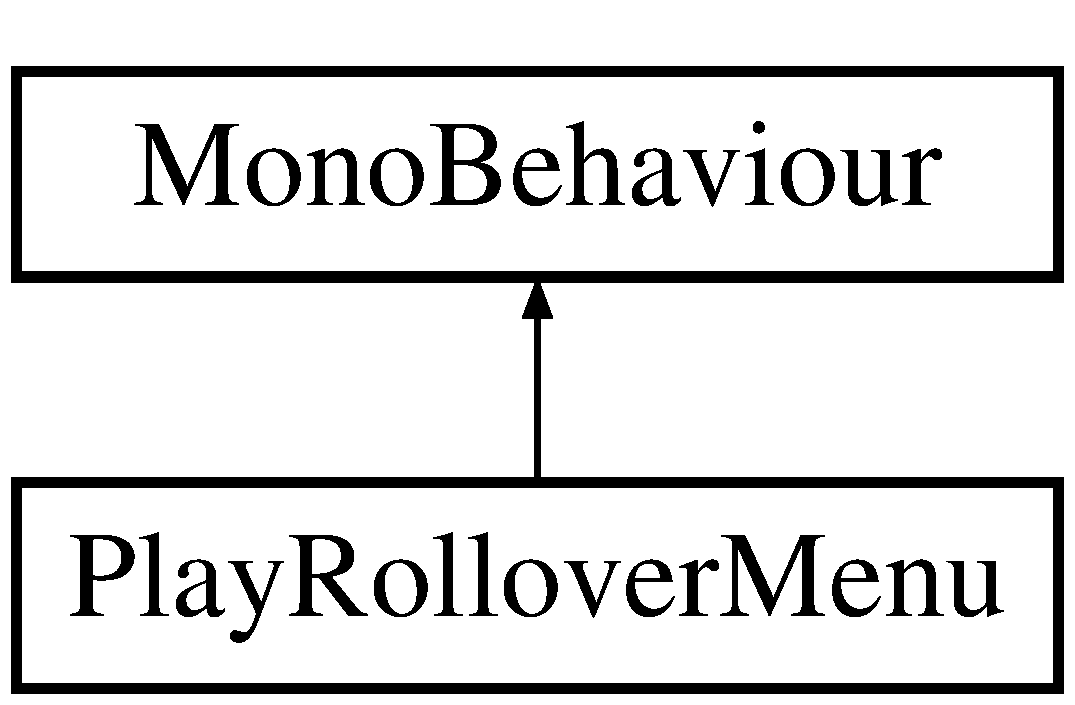
\includegraphics[height=2.000000cm]{class_play_rollover_menu}
\end{center}
\end{figure}
\subsection*{Public Attributes}
\begin{DoxyCompactItemize}
\item 
Texture2\-D \hyperlink{class_play_rollover_menu_a291ee960efe64e860a910579971d7f79}{normal\-Image}
\item 
Texture2\-D \hyperlink{class_play_rollover_menu_aa523c3e0465efefc82043c174cbf7a66}{rollover\-Image}
\end{DoxyCompactItemize}


\subsection{Detailed Description}
Interacts with the actions of the user when starting the game. 

\begin{DoxyAuthor}{Author}
David Kelly 
\end{DoxyAuthor}
\begin{DoxyVersion}{Version}
1.\-0 
\end{DoxyVersion}
\begin{DoxyDate}{Date}
20/4/14 
\end{DoxyDate}


\subsection{Member Data Documentation}
\hypertarget{class_play_rollover_menu_a291ee960efe64e860a910579971d7f79}{\index{Play\-Rollover\-Menu@{Play\-Rollover\-Menu}!normal\-Image@{normal\-Image}}
\index{normal\-Image@{normal\-Image}!PlayRolloverMenu@{Play\-Rollover\-Menu}}
\subsubsection[{normal\-Image}]{\setlength{\rightskip}{0pt plus 5cm}Texture2\-D Play\-Rollover\-Menu.\-normal\-Image}}\label{class_play_rollover_menu_a291ee960efe64e860a910579971d7f79}
Reference to image to be displayed \hypertarget{class_play_rollover_menu_aa523c3e0465efefc82043c174cbf7a66}{\index{Play\-Rollover\-Menu@{Play\-Rollover\-Menu}!rollover\-Image@{rollover\-Image}}
\index{rollover\-Image@{rollover\-Image}!PlayRolloverMenu@{Play\-Rollover\-Menu}}
\subsubsection[{rollover\-Image}]{\setlength{\rightskip}{0pt plus 5cm}Texture2\-D Play\-Rollover\-Menu.\-rollover\-Image}}\label{class_play_rollover_menu_aa523c3e0465efefc82043c174cbf7a66}
Reference to image to be displayed 

The documentation for this class was generated from the following file\-:\begin{DoxyCompactItemize}
\item 
Play\-Rollover\-Menu.\-cs\end{DoxyCompactItemize}

\hypertarget{class_rollover_game_over}{\section{Rollover\-Game\-Over Class Reference}
\label{class_rollover_game_over}\index{Rollover\-Game\-Over@{Rollover\-Game\-Over}}
}


Interacts with the actions of the user after losing all your lives.  


Inheritance diagram for Rollover\-Game\-Over\-:\begin{figure}[H]
\begin{center}
\leavevmode
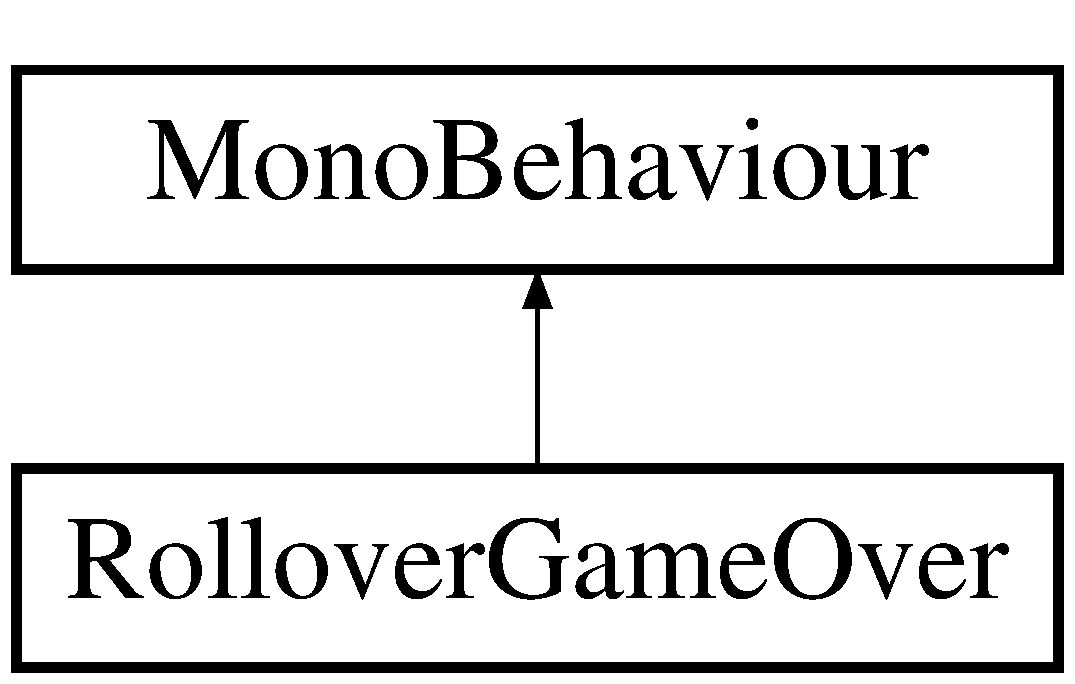
\includegraphics[height=2.000000cm]{class_rollover_game_over}
\end{center}
\end{figure}
\subsection*{Public Attributes}
\begin{DoxyCompactItemize}
\item 
Texture2\-D \hyperlink{class_rollover_game_over_ab3bb0aa666cbb2d3d5b75de7915bbaed}{normal\-Image}
\item 
Texture2\-D \hyperlink{class_rollover_game_over_a604a75ebfbcb070218d1584955d5fe76}{rollover\-Image}
\end{DoxyCompactItemize}


\subsection{Detailed Description}
Interacts with the actions of the user after losing all your lives. 

\begin{DoxyAuthor}{Author}
David Kelly 
\end{DoxyAuthor}
\begin{DoxyVersion}{Version}
1.\-0 
\end{DoxyVersion}
\begin{DoxyDate}{Date}
20/4/14 
\end{DoxyDate}


\subsection{Member Data Documentation}
\hypertarget{class_rollover_game_over_ab3bb0aa666cbb2d3d5b75de7915bbaed}{\index{Rollover\-Game\-Over@{Rollover\-Game\-Over}!normal\-Image@{normal\-Image}}
\index{normal\-Image@{normal\-Image}!RolloverGameOver@{Rollover\-Game\-Over}}
\subsubsection[{normal\-Image}]{\setlength{\rightskip}{0pt plus 5cm}Texture2\-D Rollover\-Game\-Over.\-normal\-Image}}\label{class_rollover_game_over_ab3bb0aa666cbb2d3d5b75de7915bbaed}
Reference to image to be displayed \hypertarget{class_rollover_game_over_a604a75ebfbcb070218d1584955d5fe76}{\index{Rollover\-Game\-Over@{Rollover\-Game\-Over}!rollover\-Image@{rollover\-Image}}
\index{rollover\-Image@{rollover\-Image}!RolloverGameOver@{Rollover\-Game\-Over}}
\subsubsection[{rollover\-Image}]{\setlength{\rightskip}{0pt plus 5cm}Texture2\-D Rollover\-Game\-Over.\-rollover\-Image}}\label{class_rollover_game_over_a604a75ebfbcb070218d1584955d5fe76}
Reference to image to be displayed 

The documentation for this class was generated from the following file\-:\begin{DoxyCompactItemize}
\item 
Rollover\-Game\-Over.\-cs\end{DoxyCompactItemize}

\hypertarget{class_ship_sensor}{\section{Ship\-Sensor Class Reference}
\label{class_ship_sensor}\index{Ship\-Sensor@{Ship\-Sensor}}
}


Controls whether the player collected all the parts needed to fix the ship when trigger is entered.  


Inheritance diagram for Ship\-Sensor\-:\begin{figure}[H]
\begin{center}
\leavevmode
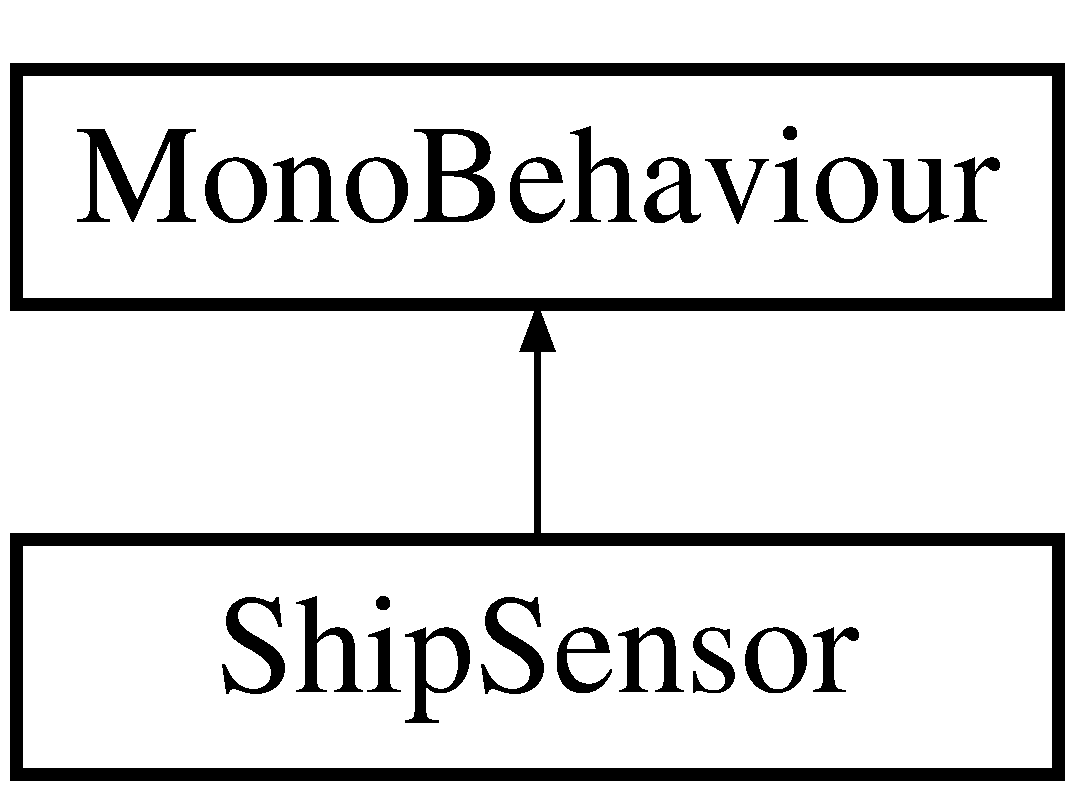
\includegraphics[height=2.000000cm]{class_ship_sensor}
\end{center}
\end{figure}
\subsection*{Public Attributes}
\begin{DoxyCompactItemize}
\item 
Game\-Object \hyperlink{class_ship_sensor_ab6f6fac60964f90237b62bfb62b8b494}{ship\-G\-O}
\item 
Audio\-Clip \hyperlink{class_ship_sensor_aef9b7a32bf81f3b3f234692315a18f12}{ship\-Start}
\item 
Game\-Object \hyperlink{class_ship_sensor_a082be7c2cb3d2ba4505d43028ffc72d3}{fading\-Message\-Prefab}
\item 
string \hyperlink{class_ship_sensor_a12336194b71d77cc4d3512fac5817ff7}{get\-Parts} = \char`\"{}(message to appear)\char`\"{}
\item 
string \hyperlink{class_ship_sensor_a8834195ac644b5dc64c7a9d6a6edc4d6}{complete} = \char`\"{}(message to appear)\char`\"{}
\end{DoxyCompactItemize}


\subsection{Detailed Description}
Controls whether the player collected all the parts needed to fix the ship when trigger is entered. 

\begin{DoxyAuthor}{Author}
David Kelly 
\end{DoxyAuthor}
\begin{DoxyVersion}{Version}
1.\-0 
\end{DoxyVersion}
\begin{DoxyDate}{Date}
20/4/14
\end{DoxyDate}
\begin{DoxyWarning}{Warning}
return values for engine parts needed from the player game object
\end{DoxyWarning}
\begin{DoxyRefDesc}{Bug}
\item[\hyperlink{bug__bug000005}{Bug}]audio is skipped when game level is loaded \end{DoxyRefDesc}


\subsection{Member Data Documentation}
\hypertarget{class_ship_sensor_a8834195ac644b5dc64c7a9d6a6edc4d6}{\index{Ship\-Sensor@{Ship\-Sensor}!complete@{complete}}
\index{complete@{complete}!ShipSensor@{Ship\-Sensor}}
\subsubsection[{complete}]{\setlength{\rightskip}{0pt plus 5cm}string Ship\-Sensor.\-complete = \char`\"{}(message to appear)\char`\"{}}}\label{class_ship_sensor_a8834195ac644b5dc64c7a9d6a6edc4d6}
Reference to the message entered \hypertarget{class_ship_sensor_a082be7c2cb3d2ba4505d43028ffc72d3}{\index{Ship\-Sensor@{Ship\-Sensor}!fading\-Message\-Prefab@{fading\-Message\-Prefab}}
\index{fading\-Message\-Prefab@{fading\-Message\-Prefab}!ShipSensor@{Ship\-Sensor}}
\subsubsection[{fading\-Message\-Prefab}]{\setlength{\rightskip}{0pt plus 5cm}Game\-Object Ship\-Sensor.\-fading\-Message\-Prefab}}\label{class_ship_sensor_a082be7c2cb3d2ba4505d43028ffc72d3}
Reference to the fading message game object \hypertarget{class_ship_sensor_a12336194b71d77cc4d3512fac5817ff7}{\index{Ship\-Sensor@{Ship\-Sensor}!get\-Parts@{get\-Parts}}
\index{get\-Parts@{get\-Parts}!ShipSensor@{Ship\-Sensor}}
\subsubsection[{get\-Parts}]{\setlength{\rightskip}{0pt plus 5cm}string Ship\-Sensor.\-get\-Parts = \char`\"{}(message to appear)\char`\"{}}}\label{class_ship_sensor_a12336194b71d77cc4d3512fac5817ff7}
Reference to the message entered \hypertarget{class_ship_sensor_ab6f6fac60964f90237b62bfb62b8b494}{\index{Ship\-Sensor@{Ship\-Sensor}!ship\-G\-O@{ship\-G\-O}}
\index{ship\-G\-O@{ship\-G\-O}!ShipSensor@{Ship\-Sensor}}
\subsubsection[{ship\-G\-O}]{\setlength{\rightskip}{0pt plus 5cm}Game\-Object Ship\-Sensor.\-ship\-G\-O}}\label{class_ship_sensor_ab6f6fac60964f90237b62bfb62b8b494}
Reference to the ship game object \hypertarget{class_ship_sensor_aef9b7a32bf81f3b3f234692315a18f12}{\index{Ship\-Sensor@{Ship\-Sensor}!ship\-Start@{ship\-Start}}
\index{ship\-Start@{ship\-Start}!ShipSensor@{Ship\-Sensor}}
\subsubsection[{ship\-Start}]{\setlength{\rightskip}{0pt plus 5cm}Audio\-Clip Ship\-Sensor.\-ship\-Start}}\label{class_ship_sensor_aef9b7a32bf81f3b3f234692315a18f12}
Reference to the audio file 

The documentation for this class was generated from the following file\-:\begin{DoxyCompactItemize}
\item 
Ship\-Sensor.\-cs\end{DoxyCompactItemize}

\hypertarget{class_third_person_camera}{\section{Third\-Person\-Camera Class Reference}
\label{class_third_person_camera}\index{Third\-Person\-Camera@{Third\-Person\-Camera}}
}
Inheritance diagram for Third\-Person\-Camera\-:\begin{figure}[H]
\begin{center}
\leavevmode
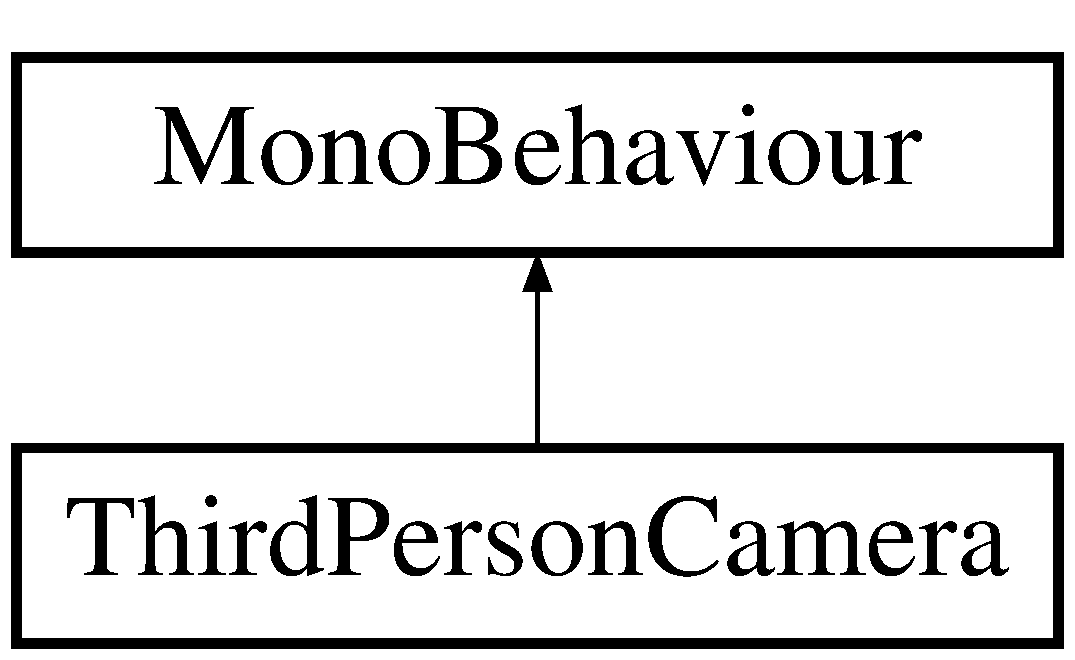
\includegraphics[height=2.000000cm]{class_third_person_camera}
\end{center}
\end{figure}
\subsection*{Public Attributes}
\begin{DoxyCompactItemize}
\item 
\hypertarget{class_third_person_camera_a93dee71af7573bcb3c3f86f39f636c72}{float {\bfseries smooth} = 3f}\label{class_third_person_camera_a93dee71af7573bcb3c3f86f39f636c72}

\end{DoxyCompactItemize}


The documentation for this class was generated from the following file\-:\begin{DoxyCompactItemize}
\item 
Third\-Person\-Camera.\-cs\end{DoxyCompactItemize}

%--- End generated contents ---

% Index
\newpage
\phantomsection
\addcontentsline{toc}{chapter}{Index}
\printindex

\end{document}
